\documentclass[a4paper,12pt]{article}
\usepackage{mathtools}
\usepackage {amsmath}
\usepackage{graphicx}
\usepackage[section]{placeins}
\usepackage{caption}
\usepackage{subcaption}
\usepackage{float}
\usepackage[a4paper, total={6.5in, 10in}]{geometry}
\usepackage{times}
\usepackage{gensymb}
\usepackage[document]{ragged2e}

\title{CSC 22100: Exercise 2}

%%% BEGIN DOCUMENT
\begin{document}

\newpage

\author{Jorge L Roldan Roldan}
\maketitle

\tableofcontents


\pagebreak
\listoffigures

\newpage
\section{Instructions}

\subsection{Part 1: Amend hierarchy of Java Classes}


\vspace{0.25cm}
Amend the hierarchy of Java classes in Exercise 1 as follows:
\vspace{0.25cm}


Polygon $is-a$ Shape; \newline
Rectangle $is-a$ Shape;  \newline
Oval $is-a$ Shape;  \newline
Circle $is-a$ Oval;  \newline

\subsection{Part 2: Interfaces}

Interface ShapeInterface, interface PositionInterface, and interface ShapePositionInterface are specified in connection with the class hierarchy.

\subsection{Part 3: ShapeInterface}


Interface ShapeInterface includes appropriate abstract, static, and/or default methods that describe the intrinsic functions and behaviors of the specific objects in the class hierarchy, including:

a. getArea $-$ describes the area of an object in the class hierarchy; \newline
b. getPerimeter $-$ describes the perimeter of an object in the class hierarchy \newline


\subsection{Part 4: PositionInterface}

Interface PositionInterface includes appropriate abstract, static, and/or default
methods that describe the positional functions and behaviors of the specific object types of the class hierarchy, including: \newpage

a. getPoint $-$ returns the point (x, y); \newline
b. moveTo $- $ moves point (x, y) to point (x + $\Delta$x, y + $\Delta$y); \newline
c. distanceTo $-$ returns distance from point (x, y) to a point 	\newline

\subsection{Part 5: ShapePositionInterface}

The abstract class Shape implements interface ShapePositionInterface which extends interface ShapeInterface and interface PositionInterface. Interface ShapePositionInterface includes appropriate abstract, static, and/or default methods that describe the functions and behaviors of the specific objects types of the class hierarchy, including: \newline
a. getBoundingBox : returns the bounding rectangle of an object in the class \newline 
hierarchy;
b. doOverlap : returns true if two objects in the class hierarchy overlap. \newline 


\subsection{Part 6: Geometric output}
Build a class Application that processes polymorphically the subclasses in the hierarchy to draw the geometric object shown:

\newpage
\section{Solution Method}

\subsection{Interfaces}
First, the three interfaces coded and their final result are shown in figures \ref{Shape interface}, \ref{Position Interface}, \ref{ShapePositionInterface} and \ref{ShapePositionInterface Part2}. The method signature they contained are specified in the instruction section above. Interface ShapePositionInterface extends the other two interfaces which is shown is line 5 using the keyword \textbf{extends}. In order to implement the method doOverlap(), the method intercept from the Shape class from javafx was used, two myClass arguments were passed to doOverlap() and the private method determineSubclass(line 11 - 35) was used to find out the subclass 
of each of the myClass objects passed to construct their respective objects from the Shape class. Doing this, the method Shape.intersect was used to determine whether two objects were overlapping.

\subsection{Classes}
For the most part, the classes remained almost the same from exercise 1. A significant difference is that myShape class (figure \ref{myShape Part1} and \ref{myShape part2}  ) is abstract since it does not implement all the abstract methods of the interfaces it implements. Some of the new methods are  moveTo  and distanceTo, whose requirements are specified in the instruction section. \newline 

\vspace{0.25cm}
Another method included in this exercise is the getBoundingBox and getPoint. These methods were implemented for classes myPolygon, myRectangle, and myOval in figures \ref{myPolygon part2}, \ref{myRectangle part1}, and \ref{myOval part2}.In order to implement getPoint, since it required to return a point data type with both x and y coordinate, a Point Class was created as shown in figure \ref{Point}.


\subsection{Polymorphism Test}
In the codes from figure \ref{DrawShapesController for Polymorphism1},\ref{DrawShapesController for Polymorphism2}, \ref{DrawShapesController for Polymorphism3}, the application built  processes polymorphically the subclasses in the hierarchy to draw the geometric object shown in the outputs sections. 


\subsection{doOverlap Test Codes}
Finally an application was built to test the performance of doOverlap method. This code is include in figures \ref{DrawShapesController for doOverlap1} ,\ref{DrawShapesController for doOverlap2}, \ref{DrawShapesController for doOverlap3}.


\section{Codes developed}

\subsection{Interfaces Codes}
\begin{figure}[H]
   \centering
   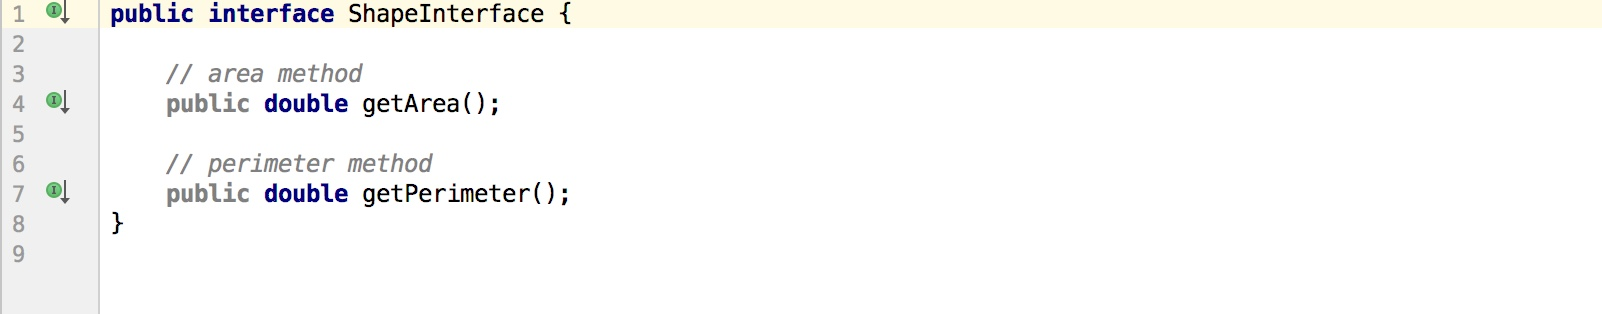
\includegraphics[width = 17cm]{shape_interface} % requires the graphicx package
   \caption{Shape interface}
   \label{Shape interface}
\end{figure}

\begin{figure}[H]
   \centering
   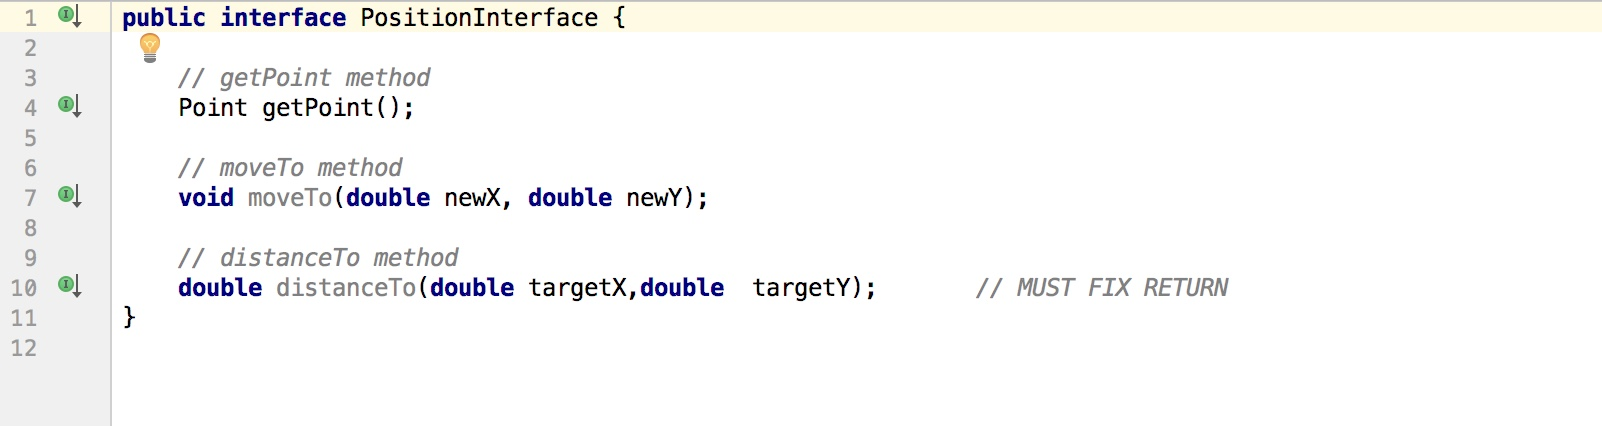
\includegraphics[width = 17cm]{PositionInterface} % requires the graphicx package
   \caption{Position Interface}
   \label{Position Interface}
\end{figure}

\begin{figure}[H]
   \centering
   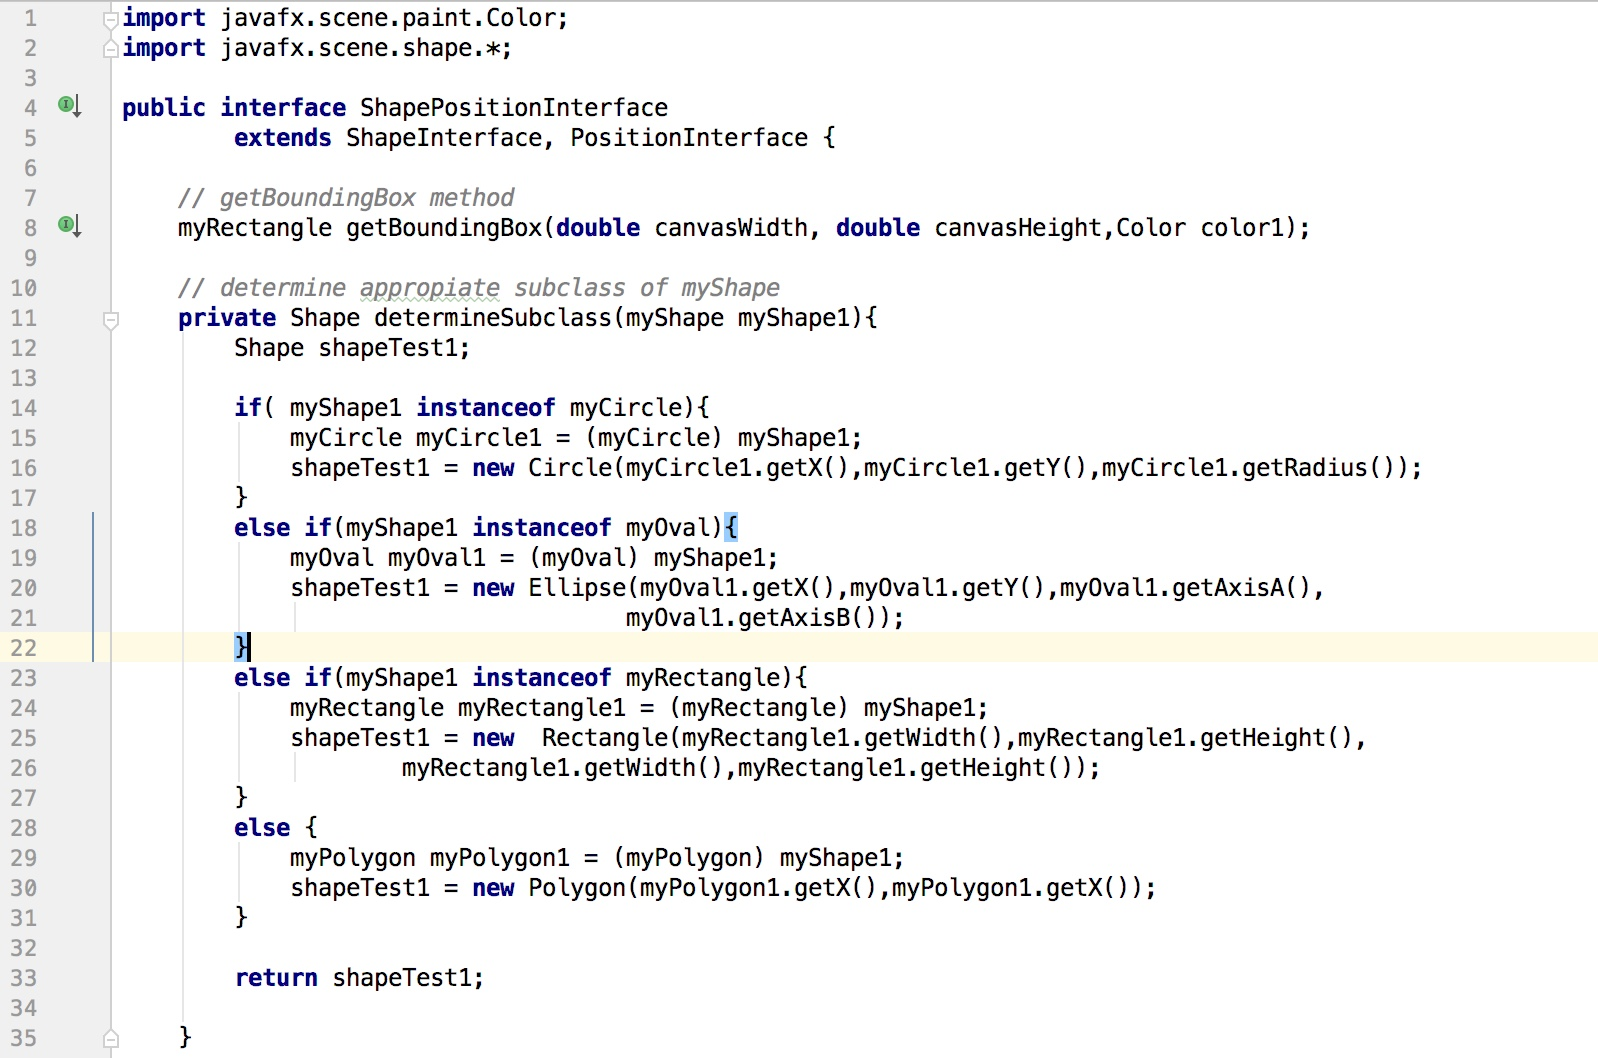
\includegraphics[width = 17cm]{ShapePositionInterface} % requires the graphicx package
   \caption{ShapePositionInterface}
   \label{ShapePositionInterface}
\end{figure}


\begin{figure}[H]
   \centering
   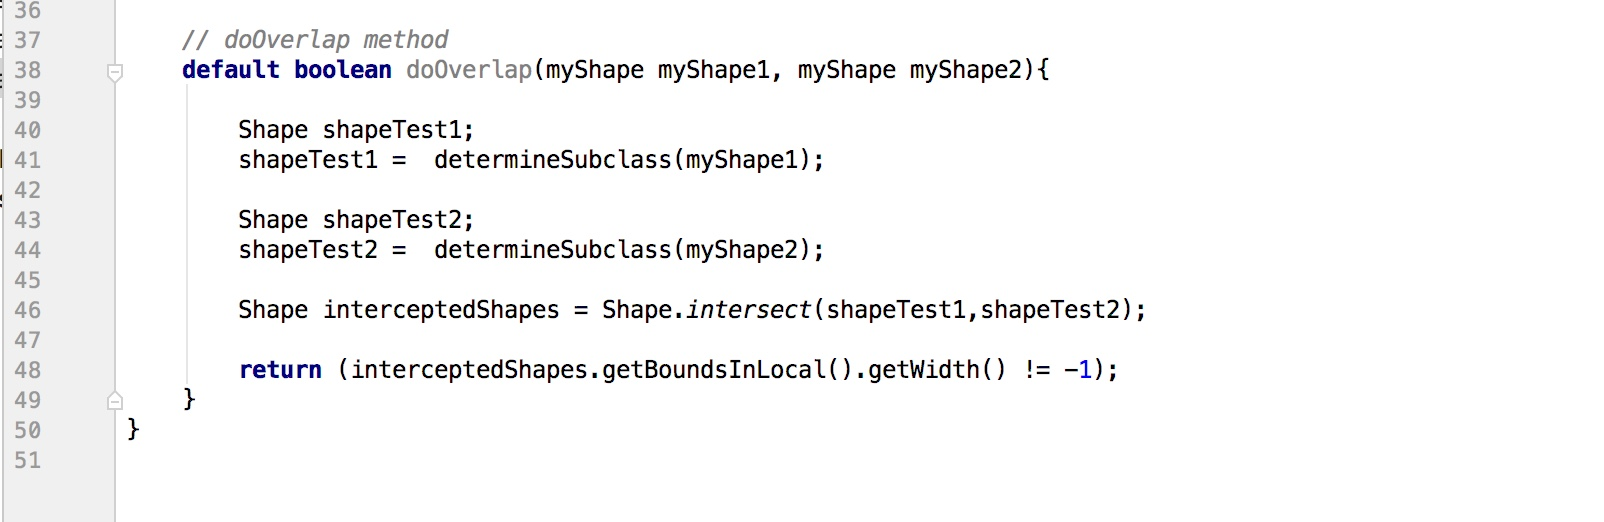
\includegraphics[width = 17cm]{ShapePositionInterface_part2} % requires the graphicx package
   \caption{ShapePositionInterface Part2}
   \label{ShapePositionInterface Part2}
\end{figure}

\subsection{Classes Codes}

\begin{figure}[H]
   \centering
   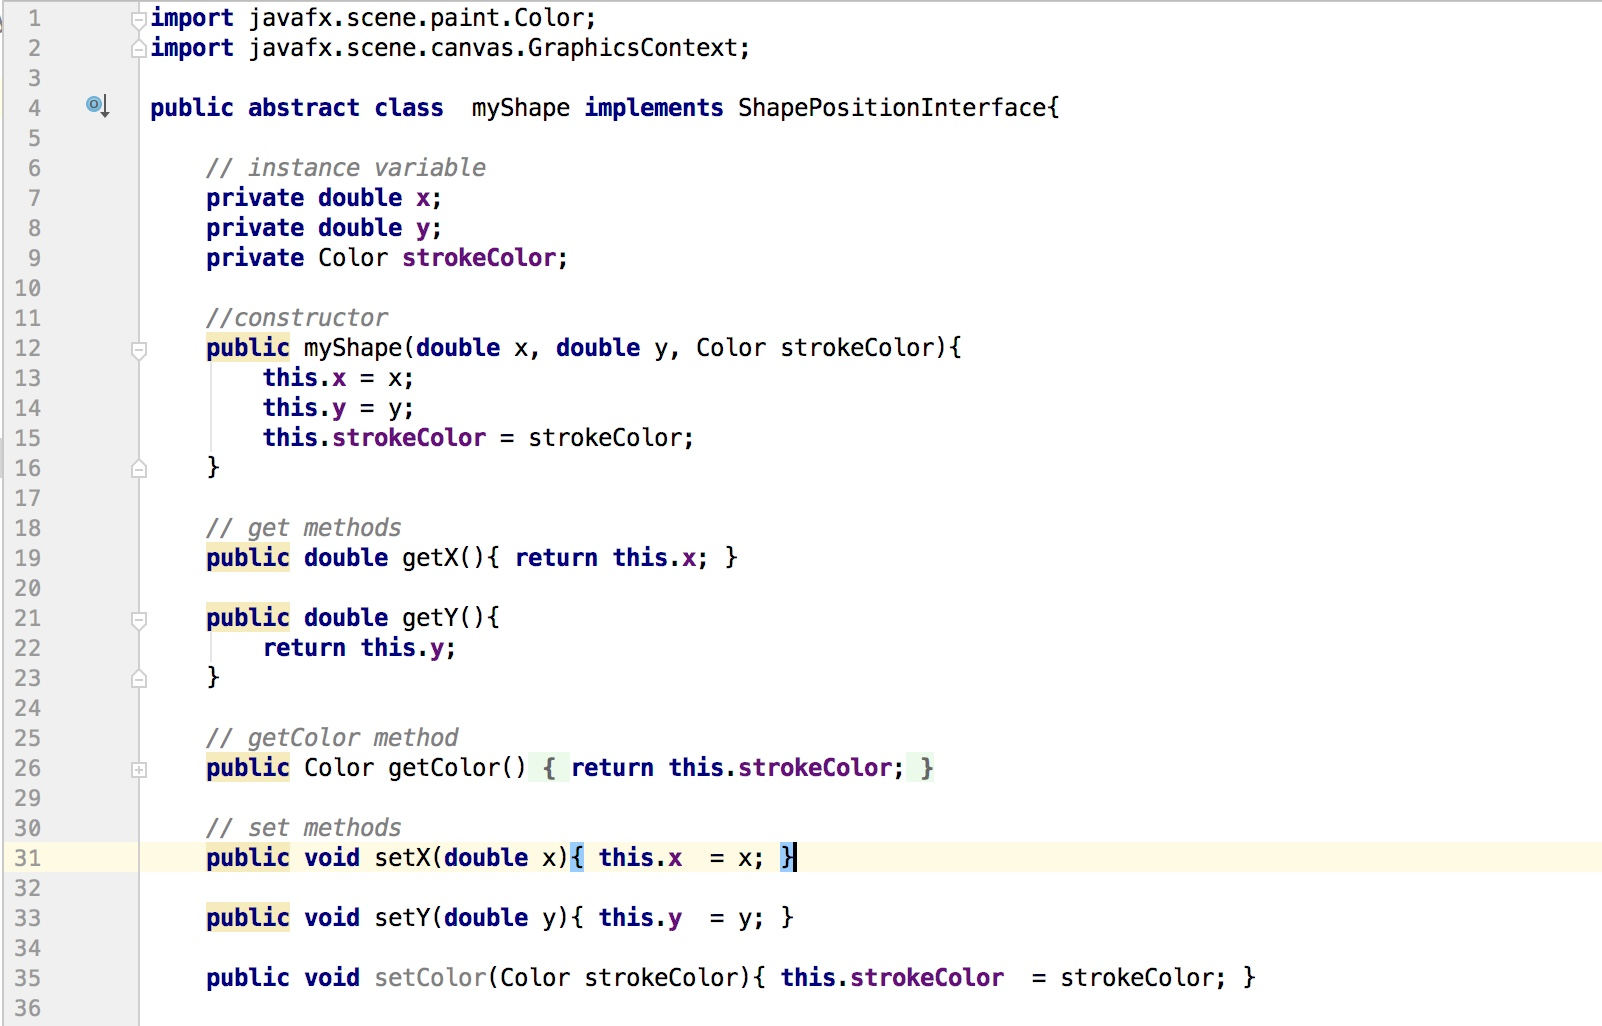
\includegraphics[width = 17cm]{myShape_part1} % requires the graphicx package
   \caption{myShape Part1}
   \label{myShape Part1}
\end{figure}


\begin{figure}[H]
   \centering
   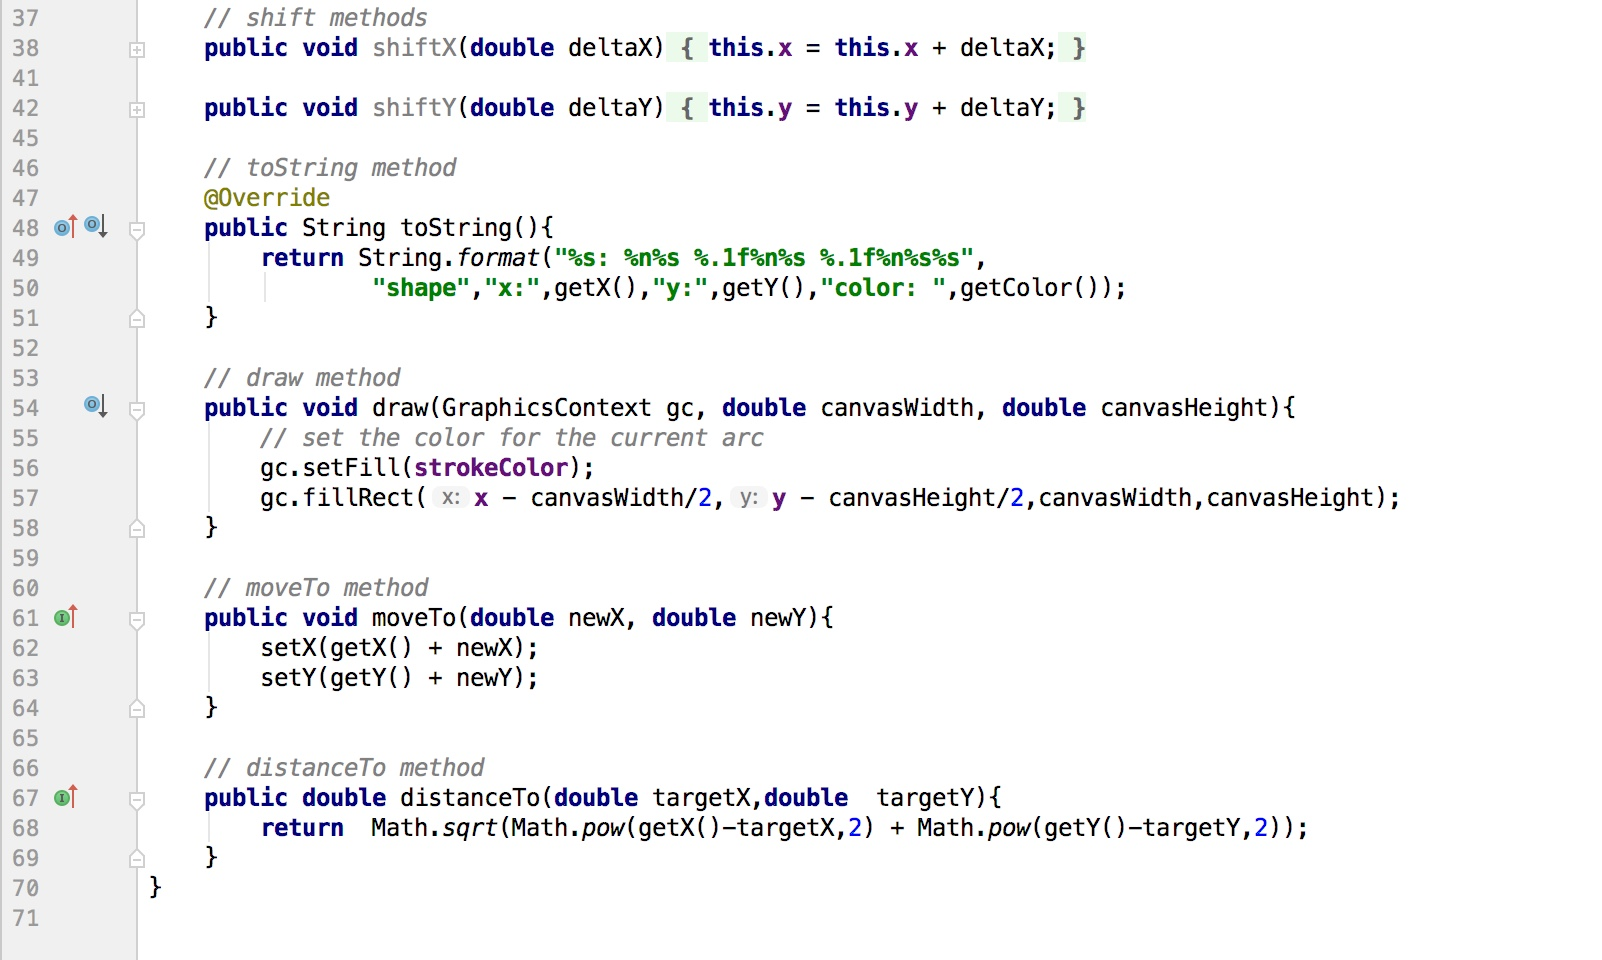
\includegraphics[width = 17cm]{myShape_part2} % requires the graphicx package
   \caption{myShape part2}
   \label{myShape part2}
\end{figure}


\begin{figure}[H]
   \centering
   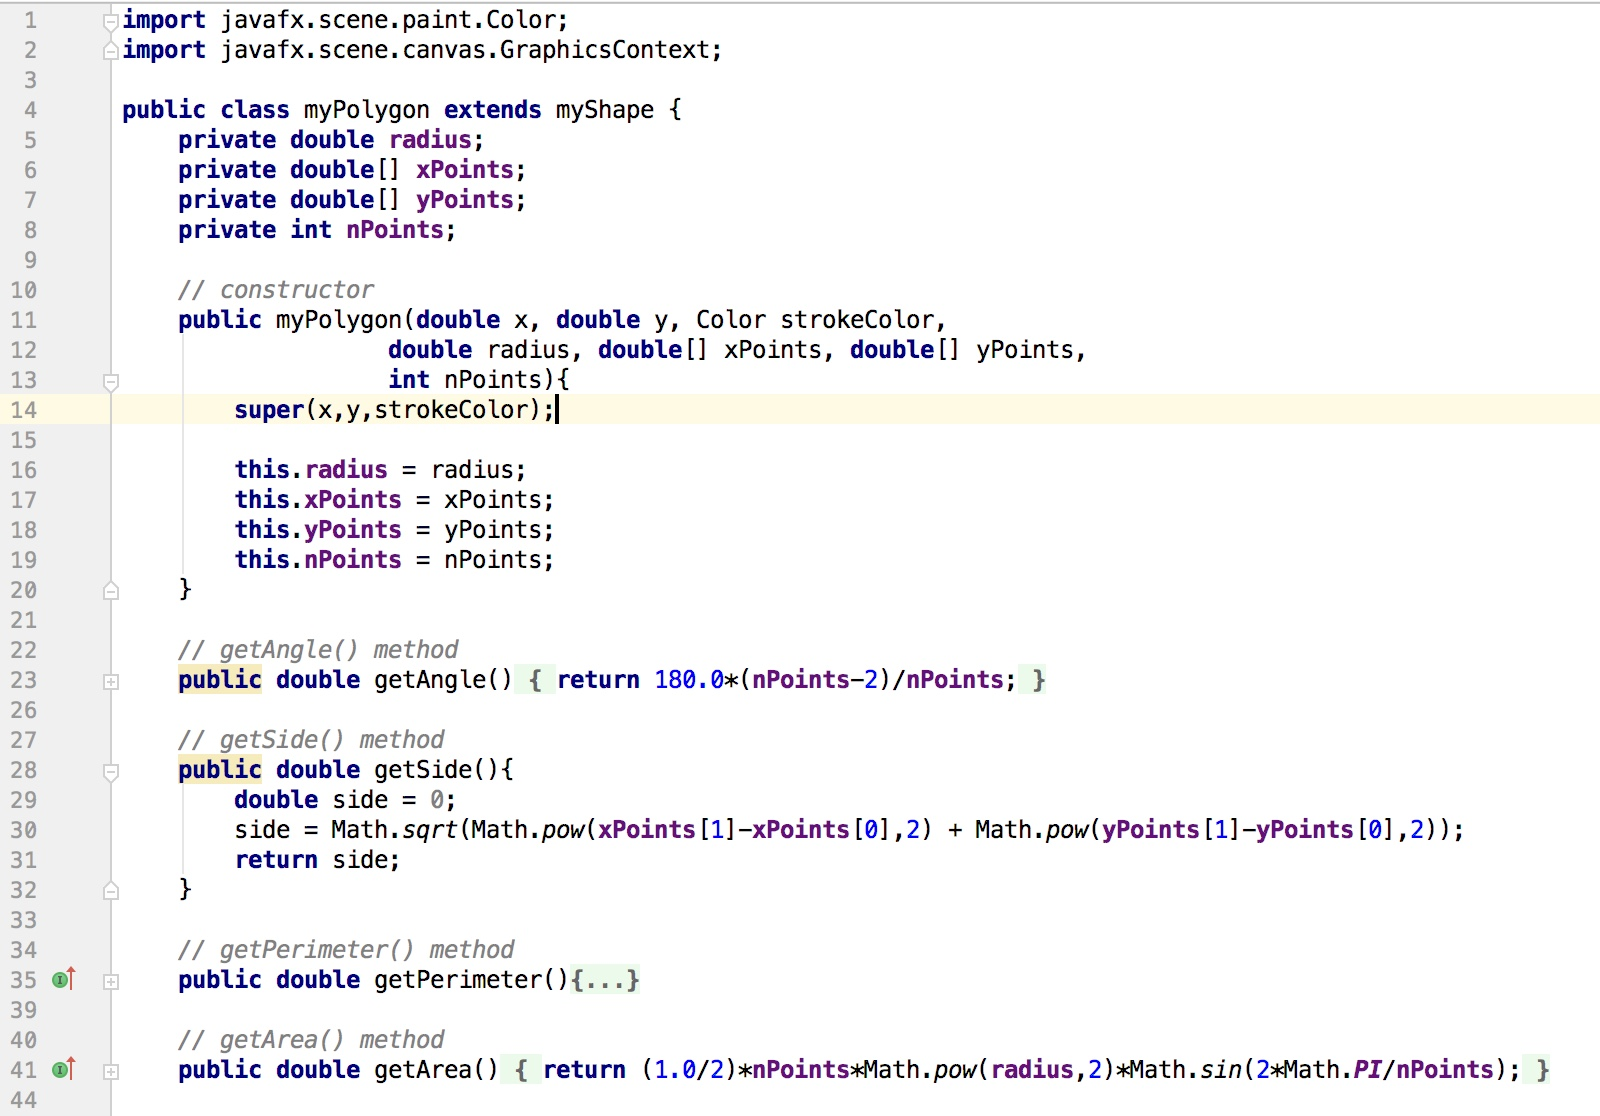
\includegraphics[width = 17cm]{myPolygon_part1} % requires the graphicx package
   \caption{myPolygon part1}
   \label{myPolygon part1}
\end{figure}




\begin{figure}[H]
   \centering
   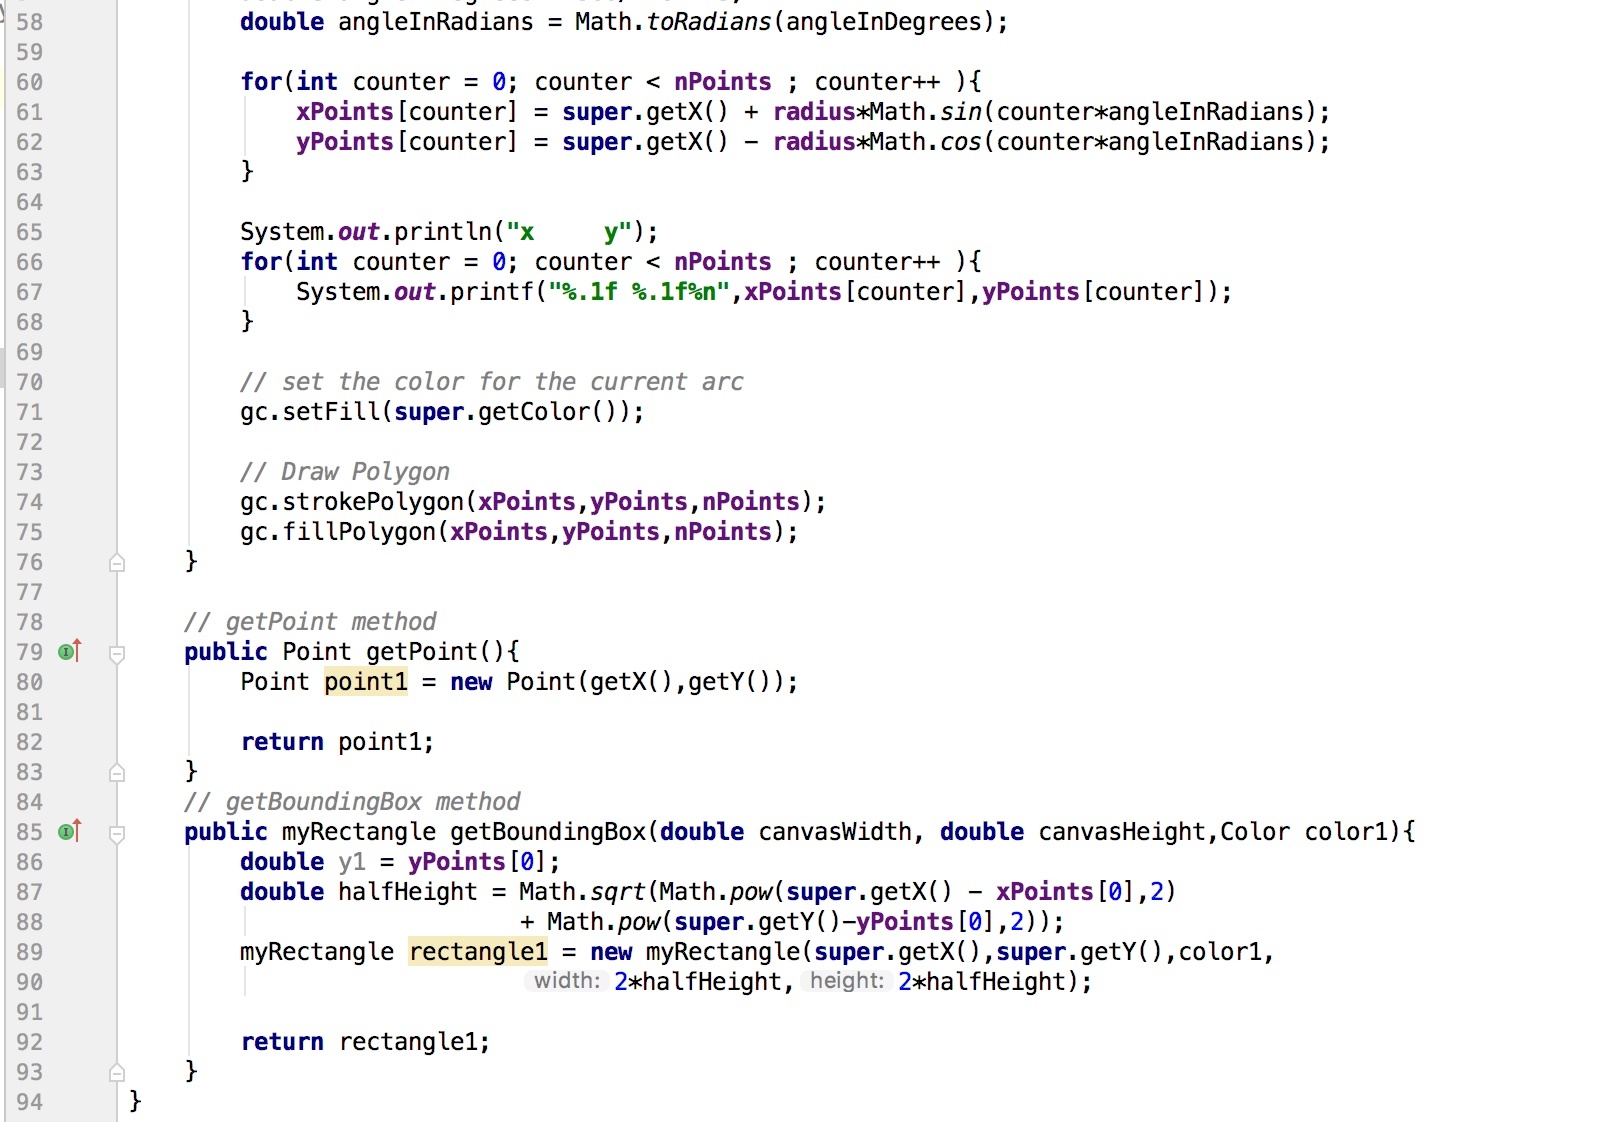
\includegraphics[width = 17cm]{myPolygon_part2} % requires the graphicx package
   \caption{myPolygon part2}
   \label{myPolygon part2}
\end{figure}


\begin{figure}[H]
   \centering
   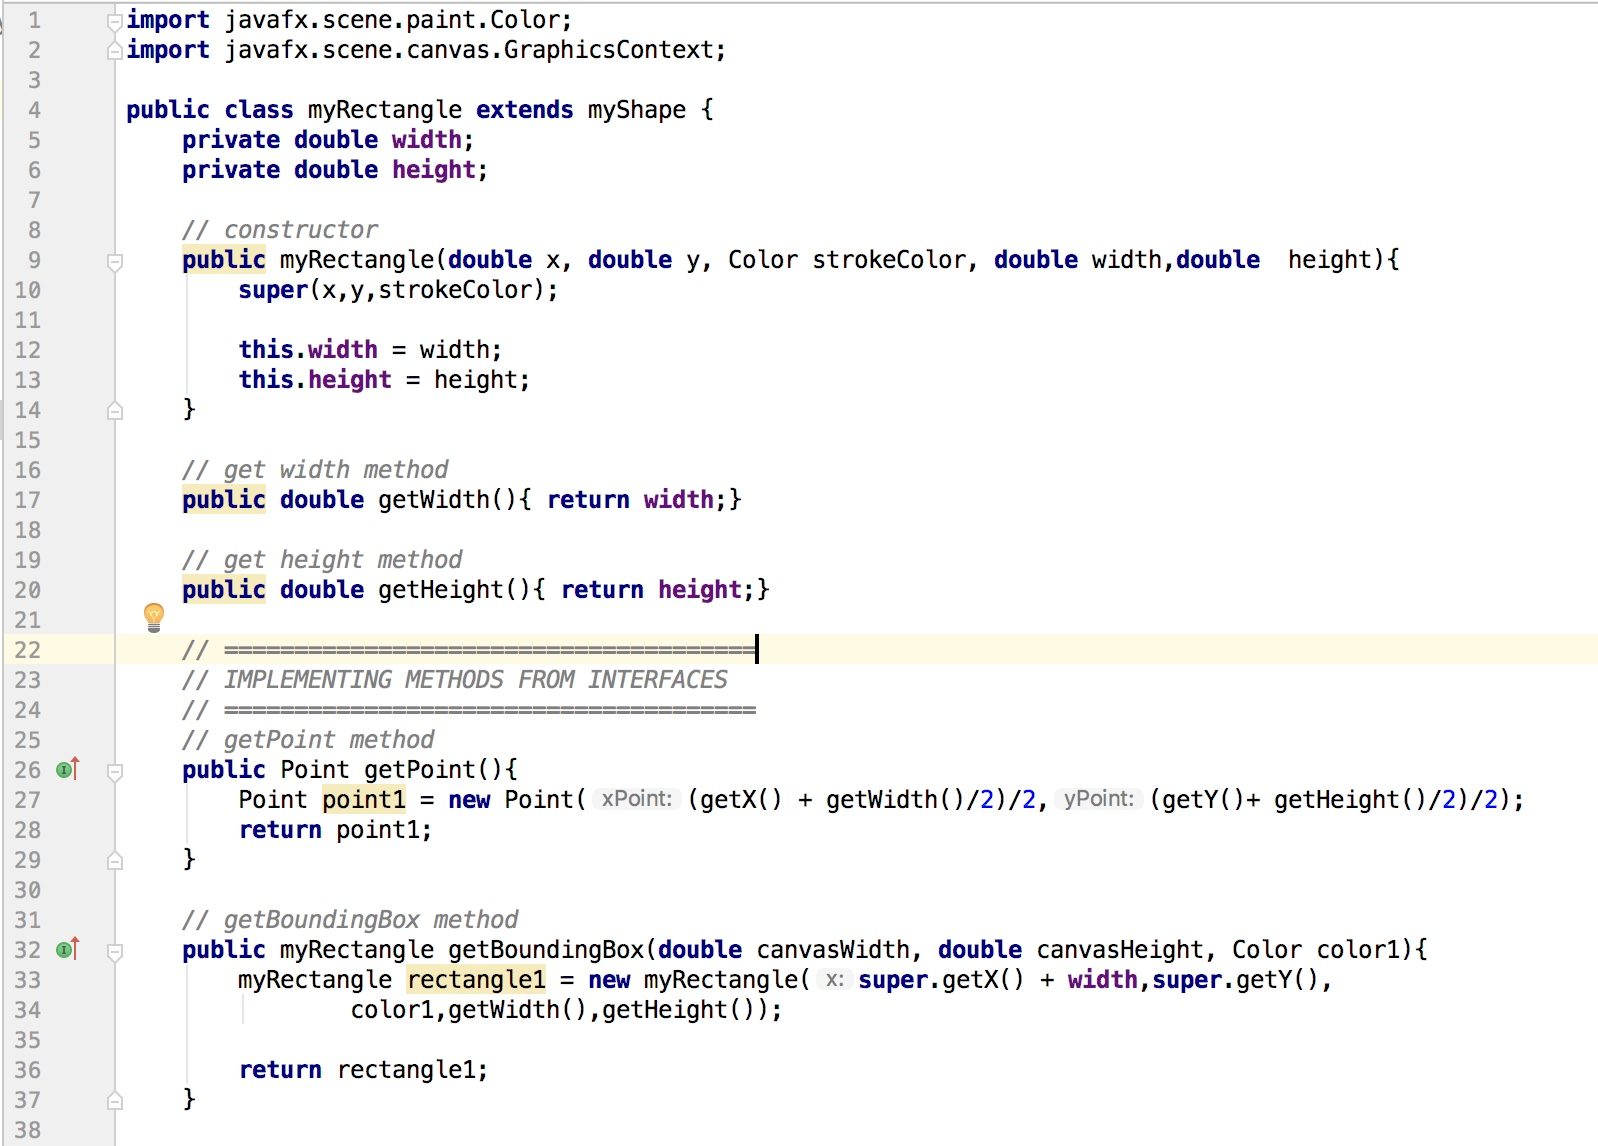
\includegraphics[width = 17cm]{myRectangle_part1} % requires the graphicx package
   \caption{myRectangle part1}
   \label{myRectangle part1}
\end{figure}



\begin{figure}[H]
   \centering
   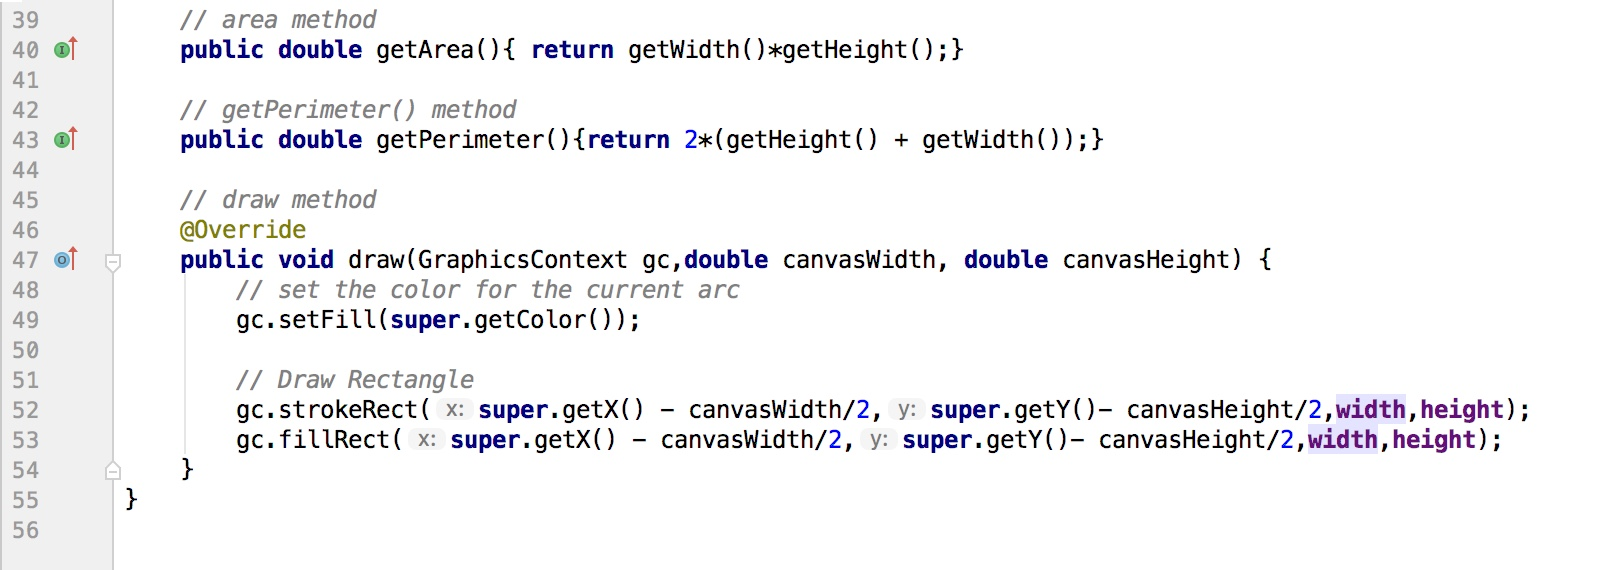
\includegraphics[width = 17cm]{myRectangle_part2} % requires the graphicx package
   \caption{myRectangle part2}
   \label{myRectangle part2}
\end{figure}


\begin{figure}[H]
   \centering
   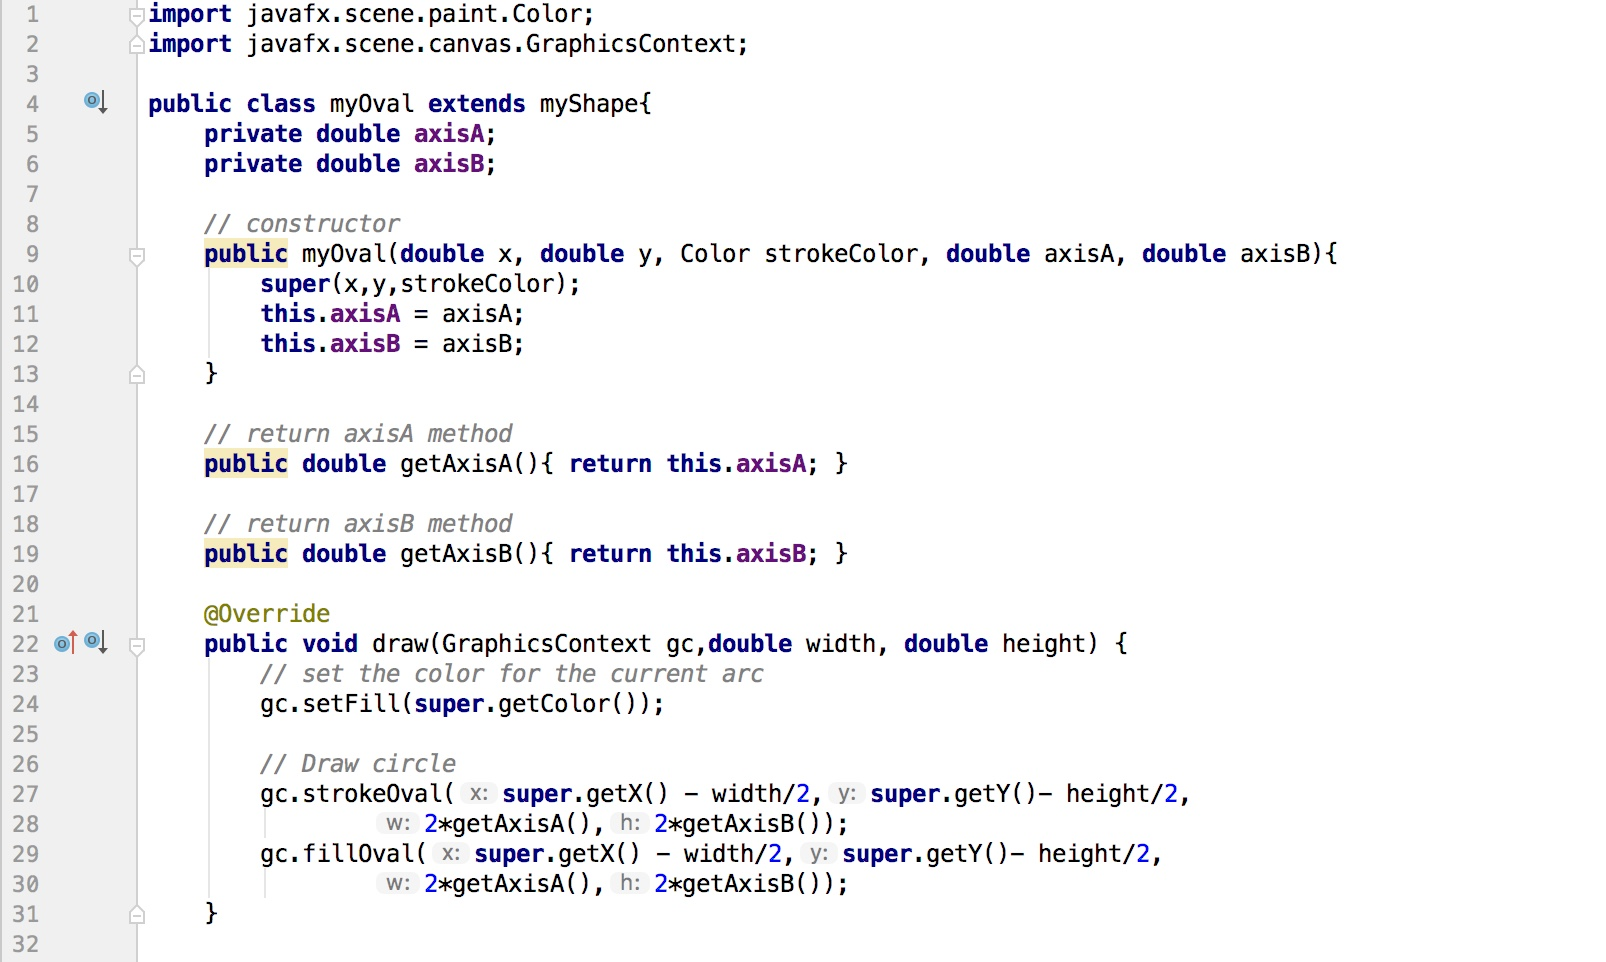
\includegraphics[width = 17cm]{myOval_part1} % requires the graphicx package
   \caption{myOval part1}
   \label{myOval part1}
\end{figure}



\begin{figure}[H]
   \centering
   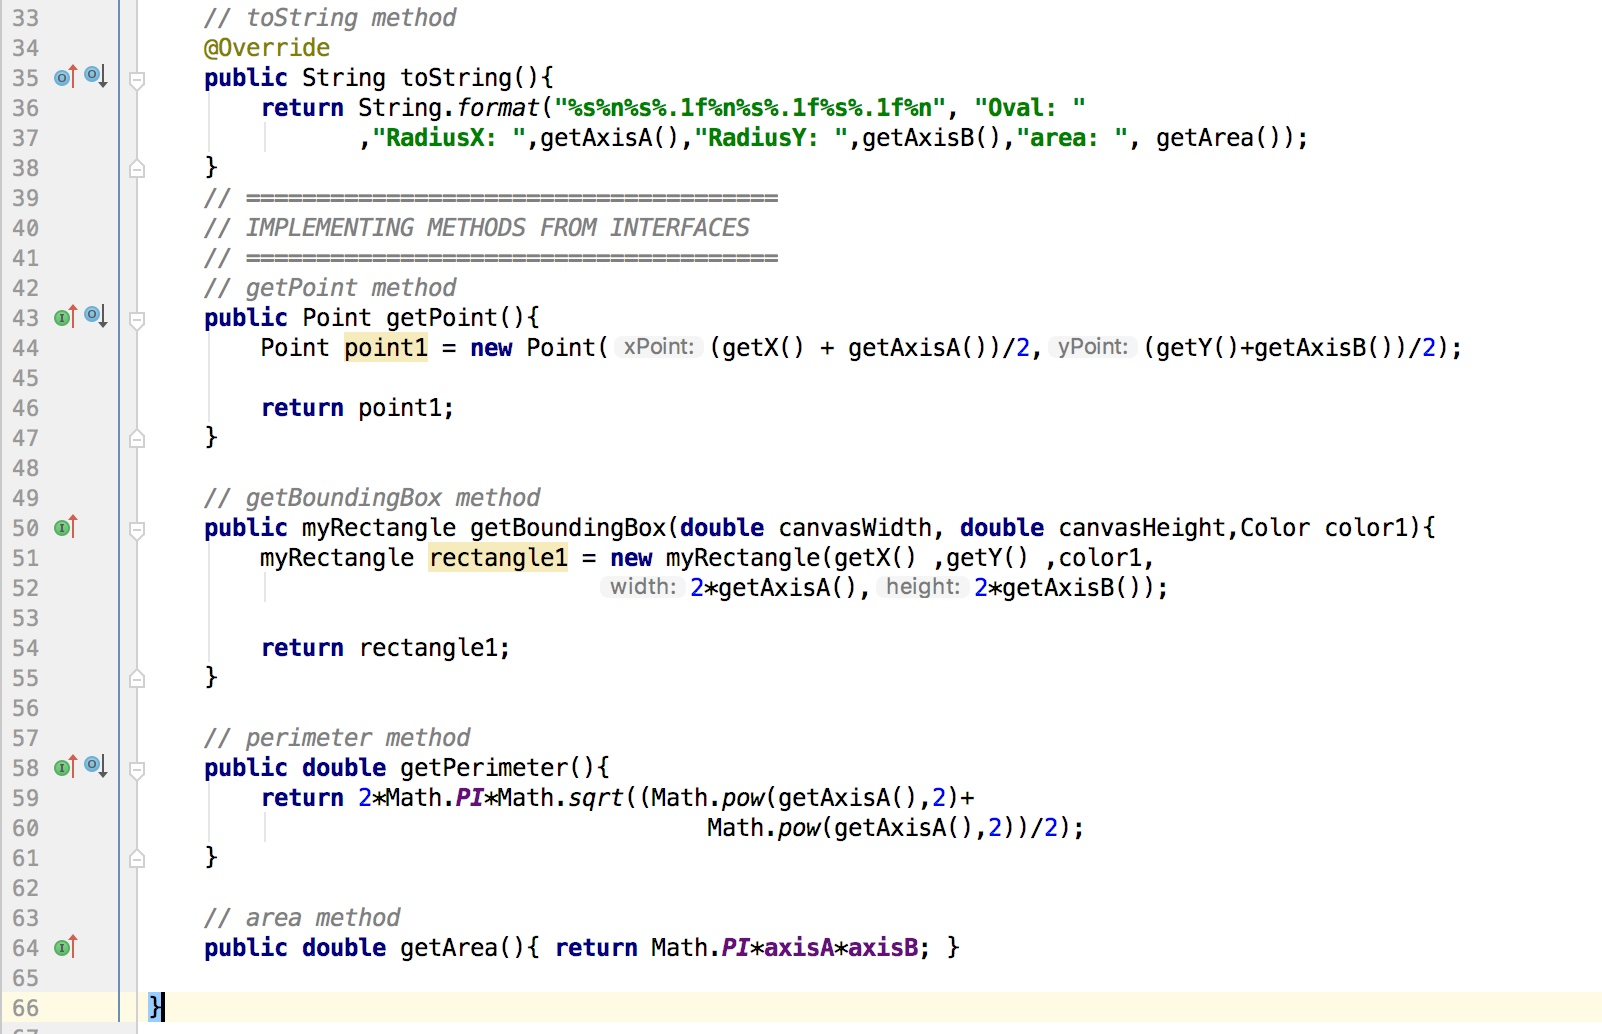
\includegraphics[width = 17cm]{myOval_part2} % requires the graphicx package
   \caption{myOval part2}
   \label{myOval part2}
\end{figure}


\begin{figure}[H]
   \centering
   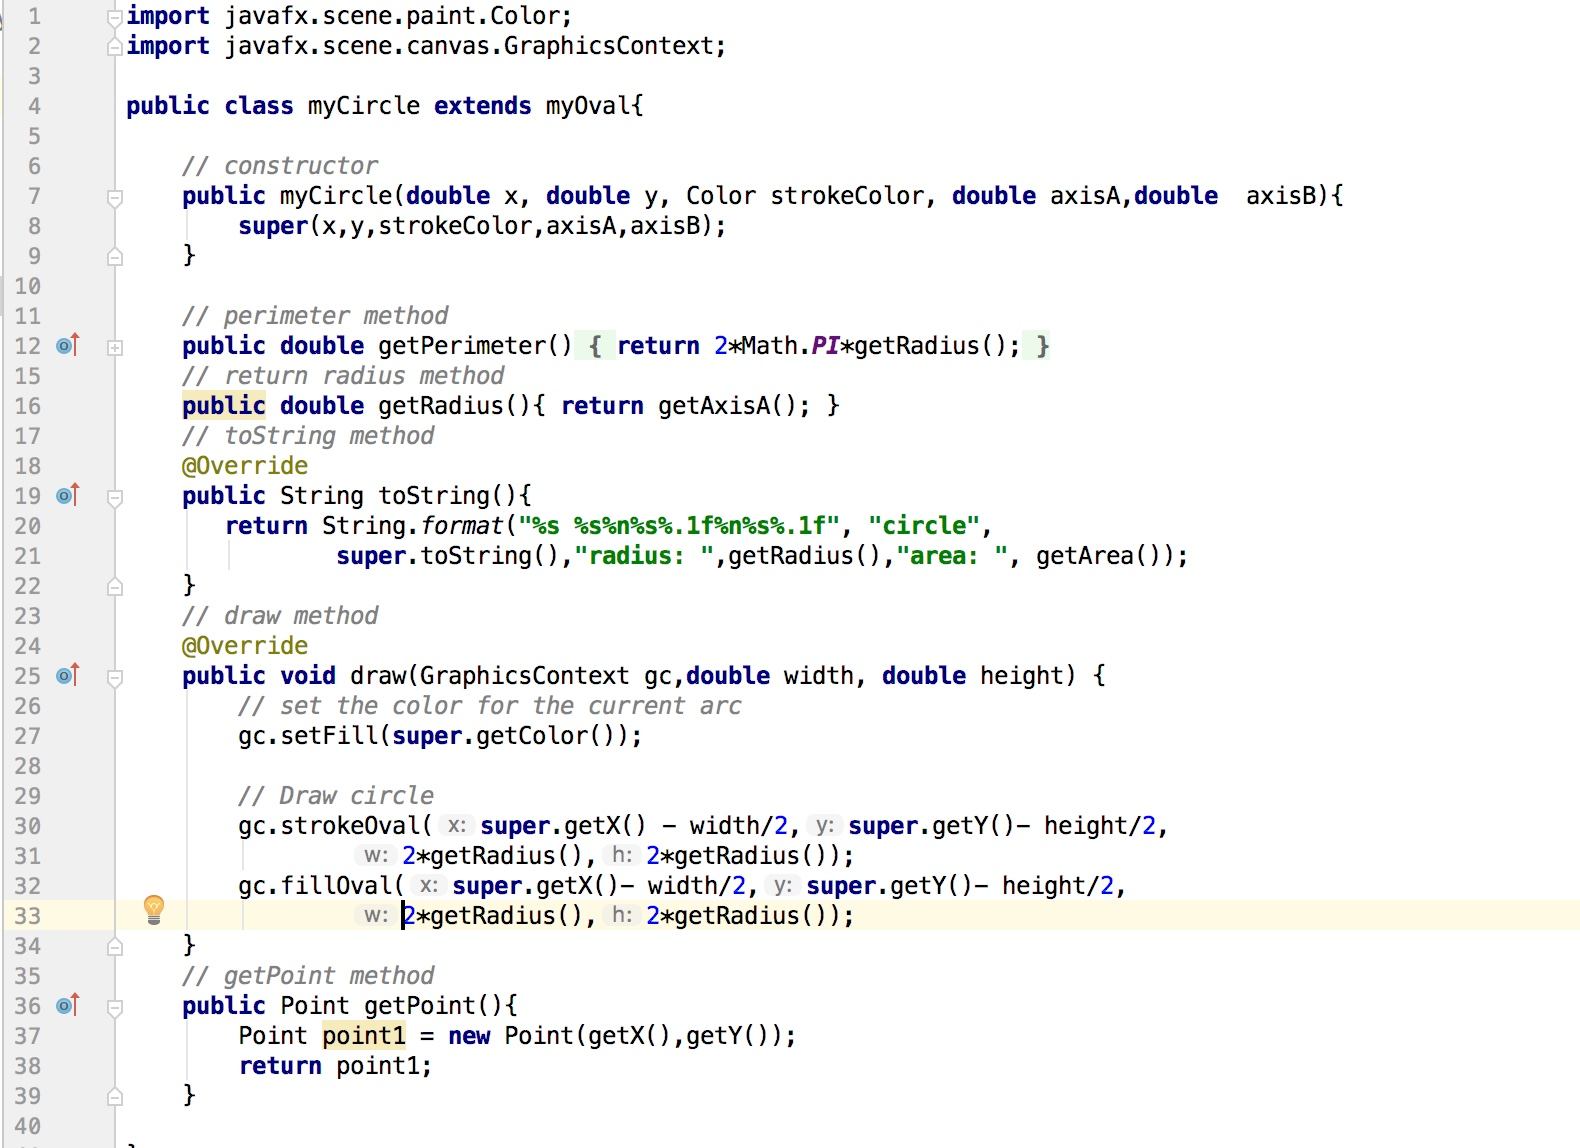
\includegraphics[width = 17cm]{myCircle} % requires the graphicx package
   \caption{myCircle}
   \label{myCircle}
\end{figure}


\begin{figure}[H]
   \centering
   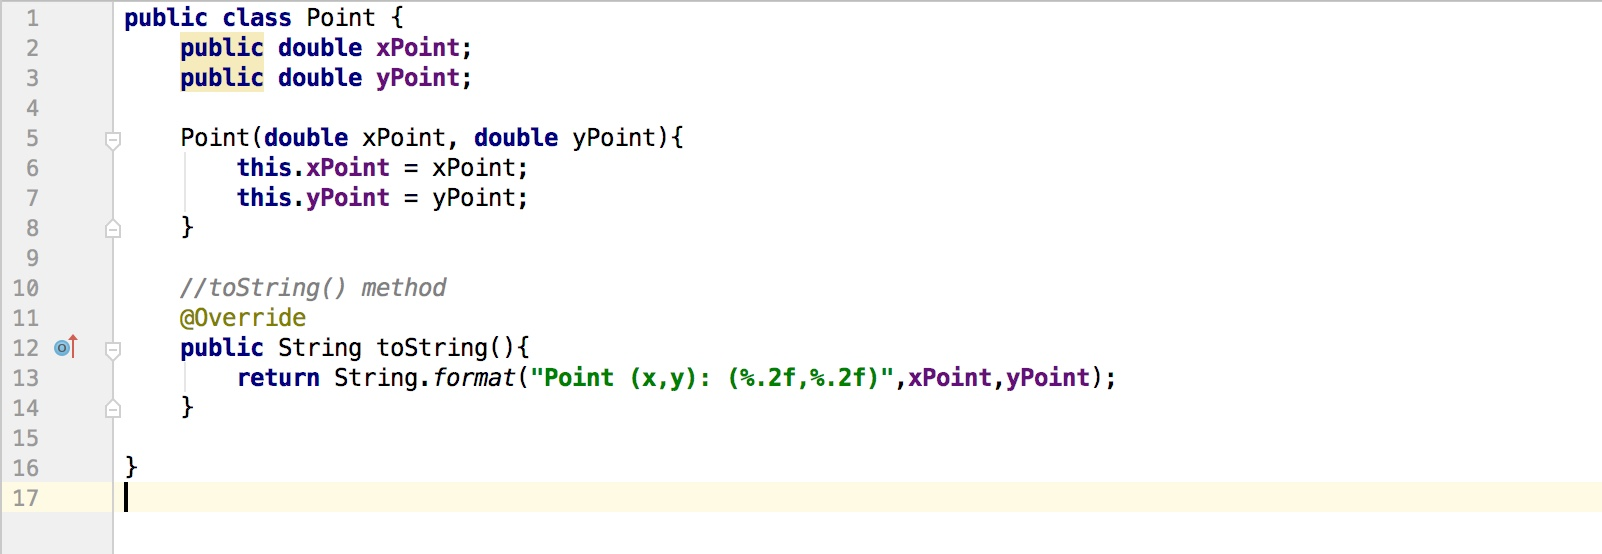
\includegraphics[width = 17cm]{Point} % requires the graphicx package
   \caption{Point}
   \label{Point}
\end{figure}

\subsection{Polymorphism Test Codes}
\begin{figure}[H]
   \centering
   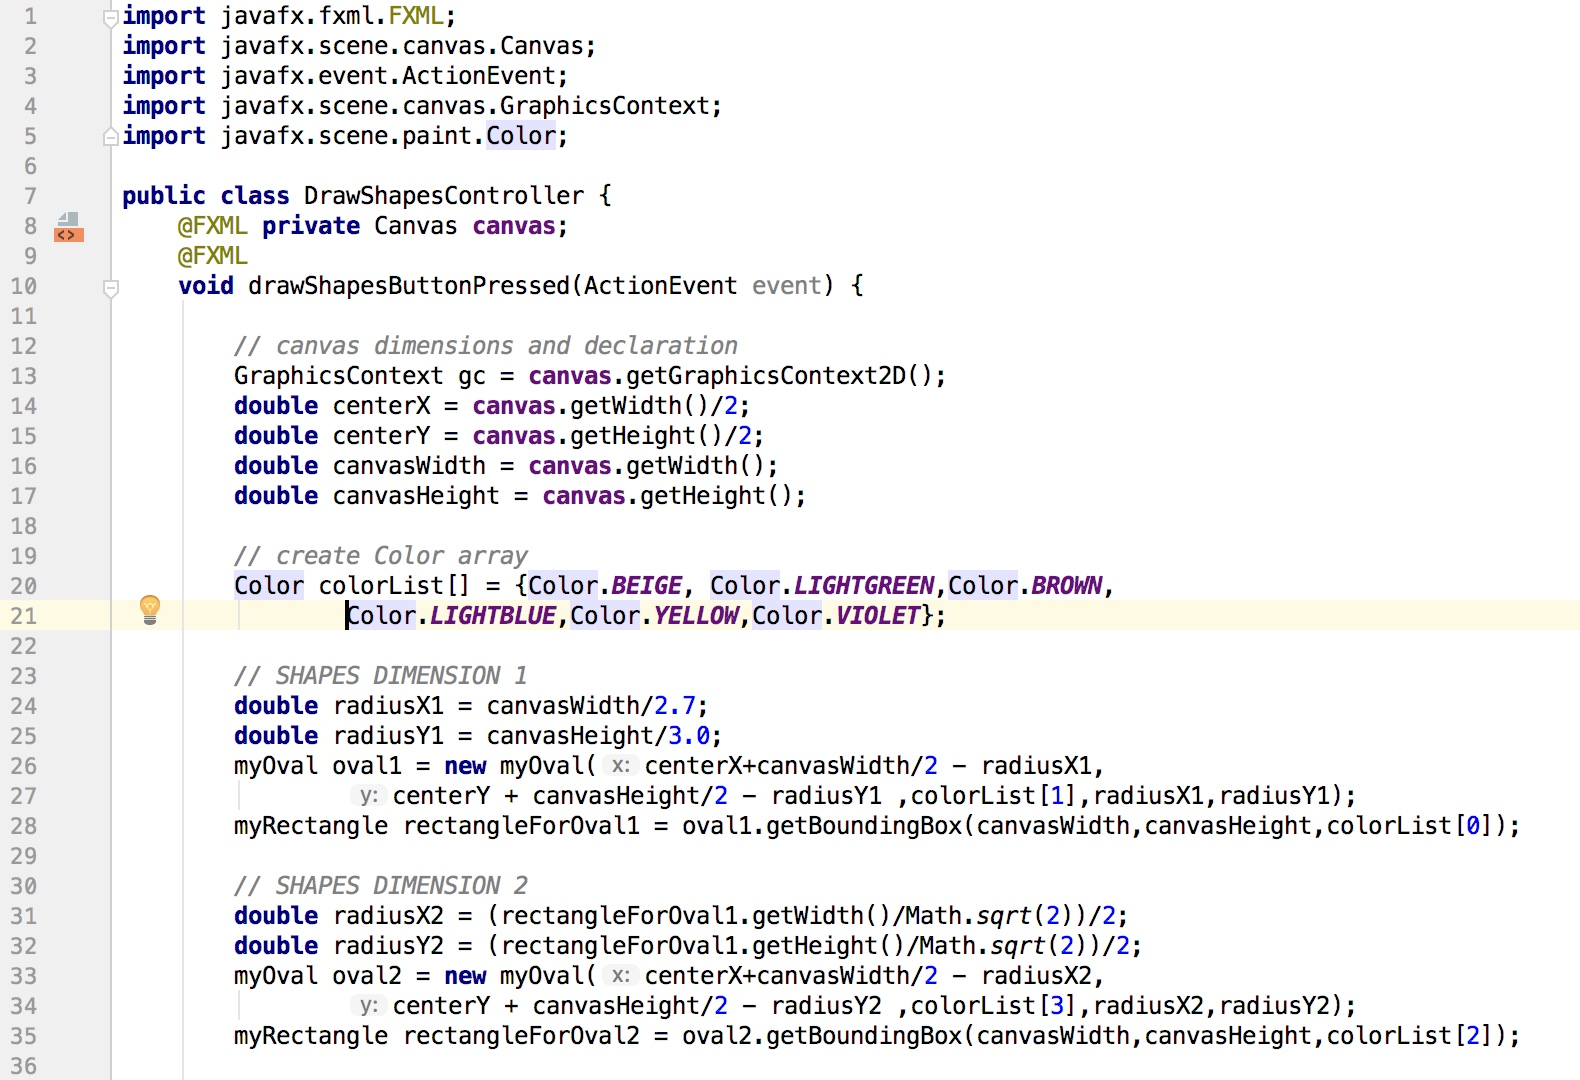
\includegraphics[width = 17cm]{Test_for_Polymorphism_part1} % requires the graphicx package
   \caption{DrawShapesController for Polymorphism1}
   \label{DrawShapesController for Polymorphism1}
\end{figure}


\begin{figure}[H]
   \centering
   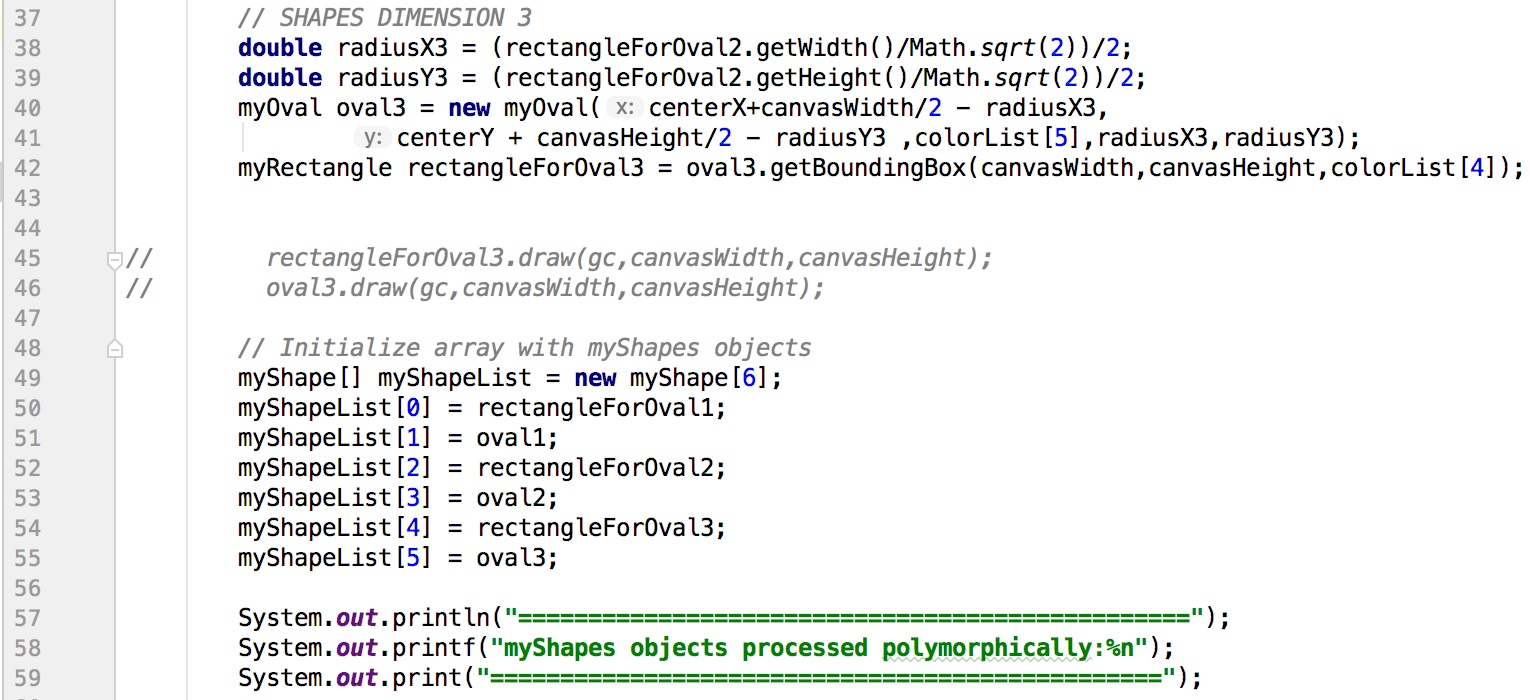
\includegraphics[width = 17cm]{Test_for_Polymorphism_part2} % requires the graphicx package
   \caption{DrawShapesController for Polymorphism2}
   \label{DrawShapesController for Polymorphism2}
\end{figure}

\begin{figure}[H]
   \centering
   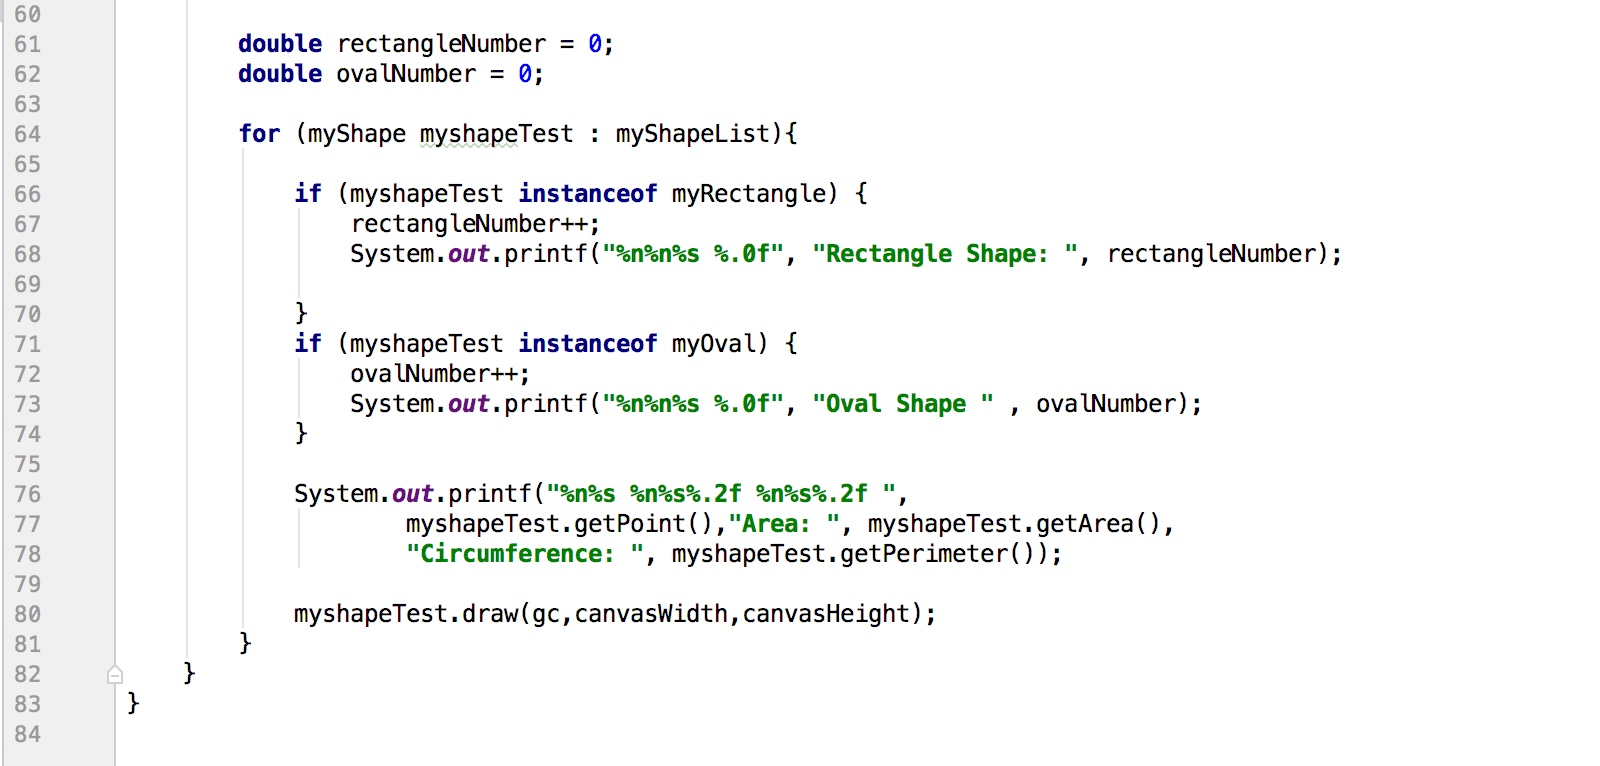
\includegraphics[width = 17cm]{Test_for_Polymorphism_part3} % requires the graphicx package
   \caption{DrawShapesController for Polymorphism3}
   \label{DrawShapesController for Polymorphism3}
\end{figure}


\subsection{doOverlap Test Codes}

\begin{figure}[H]
   \centering
   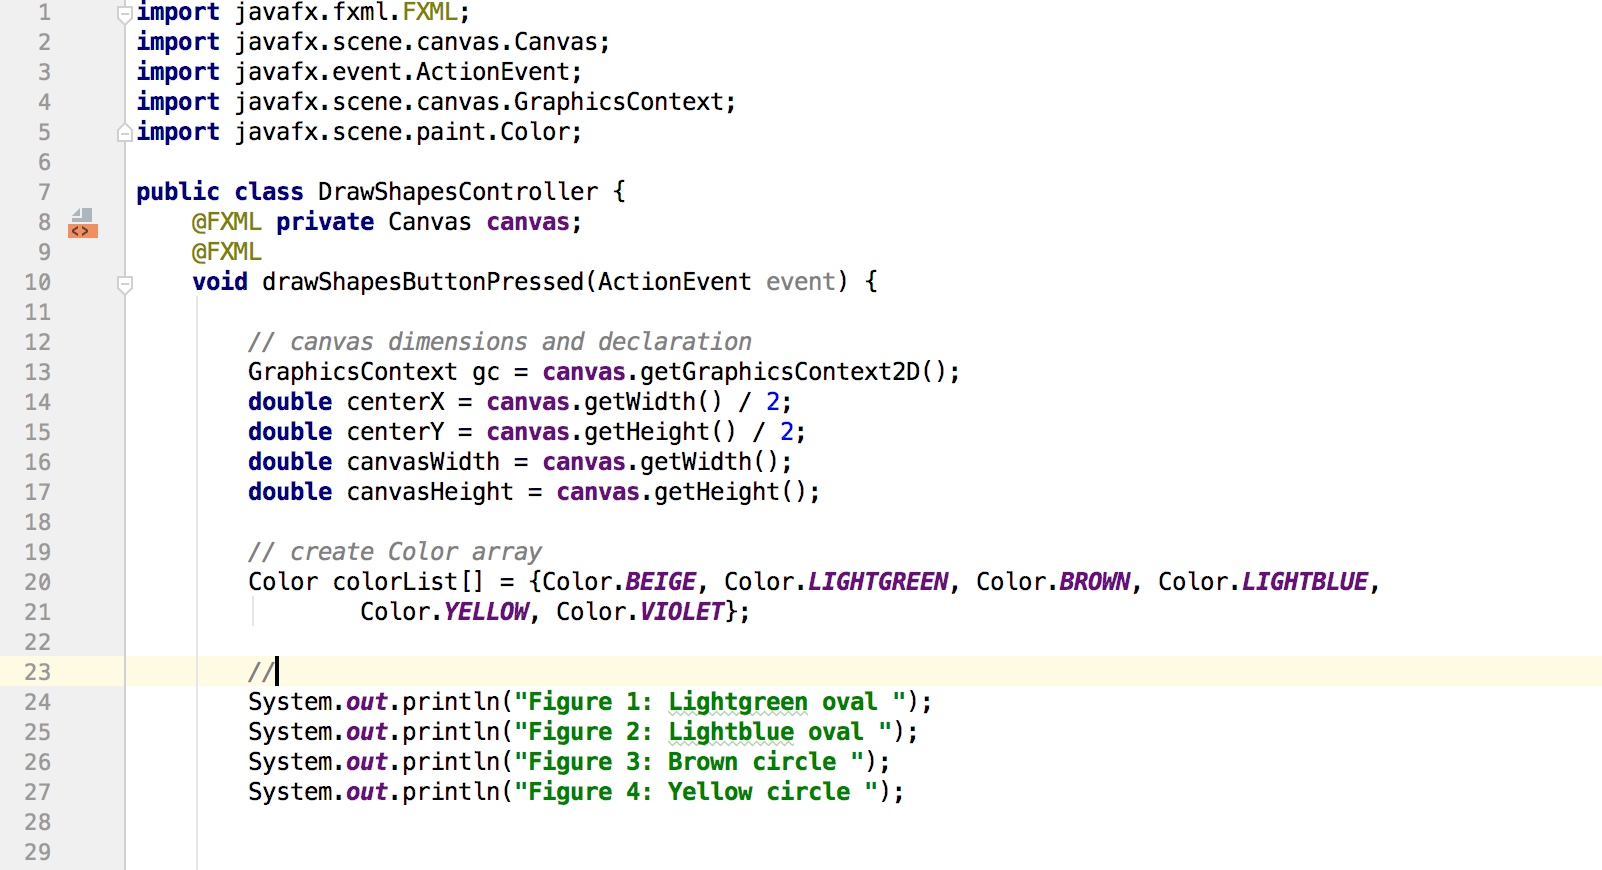
\includegraphics[width = 17cm]{DrawShapesController_for_doOverlap1} % requires the graphicx package
   \caption{DrawShapesController for doOverlap1}
   \label{DrawShapesController for doOverlap1}
\end{figure}


\begin{figure}[H]
   \centering
   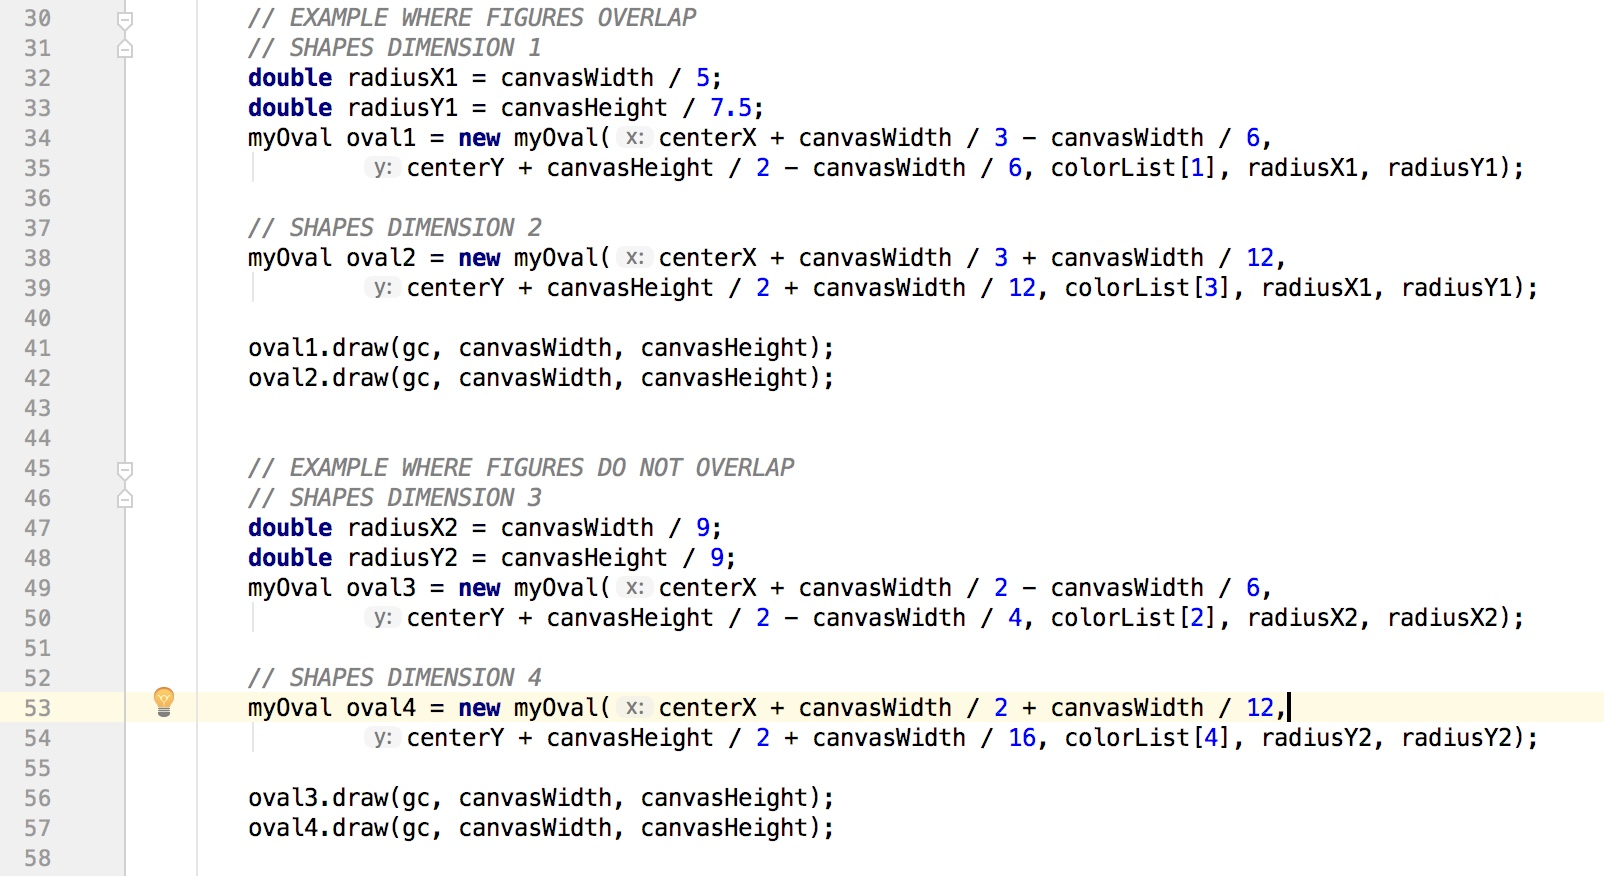
\includegraphics[width = 17cm]{DrawShapesController_for_doOverlap2} % requires the graphicx package
   \caption{DrawShapesController for doOverlap2}
   \label{DrawShapesController for doOverlap2}
\end{figure}


\begin{figure}[H]
   \centering
   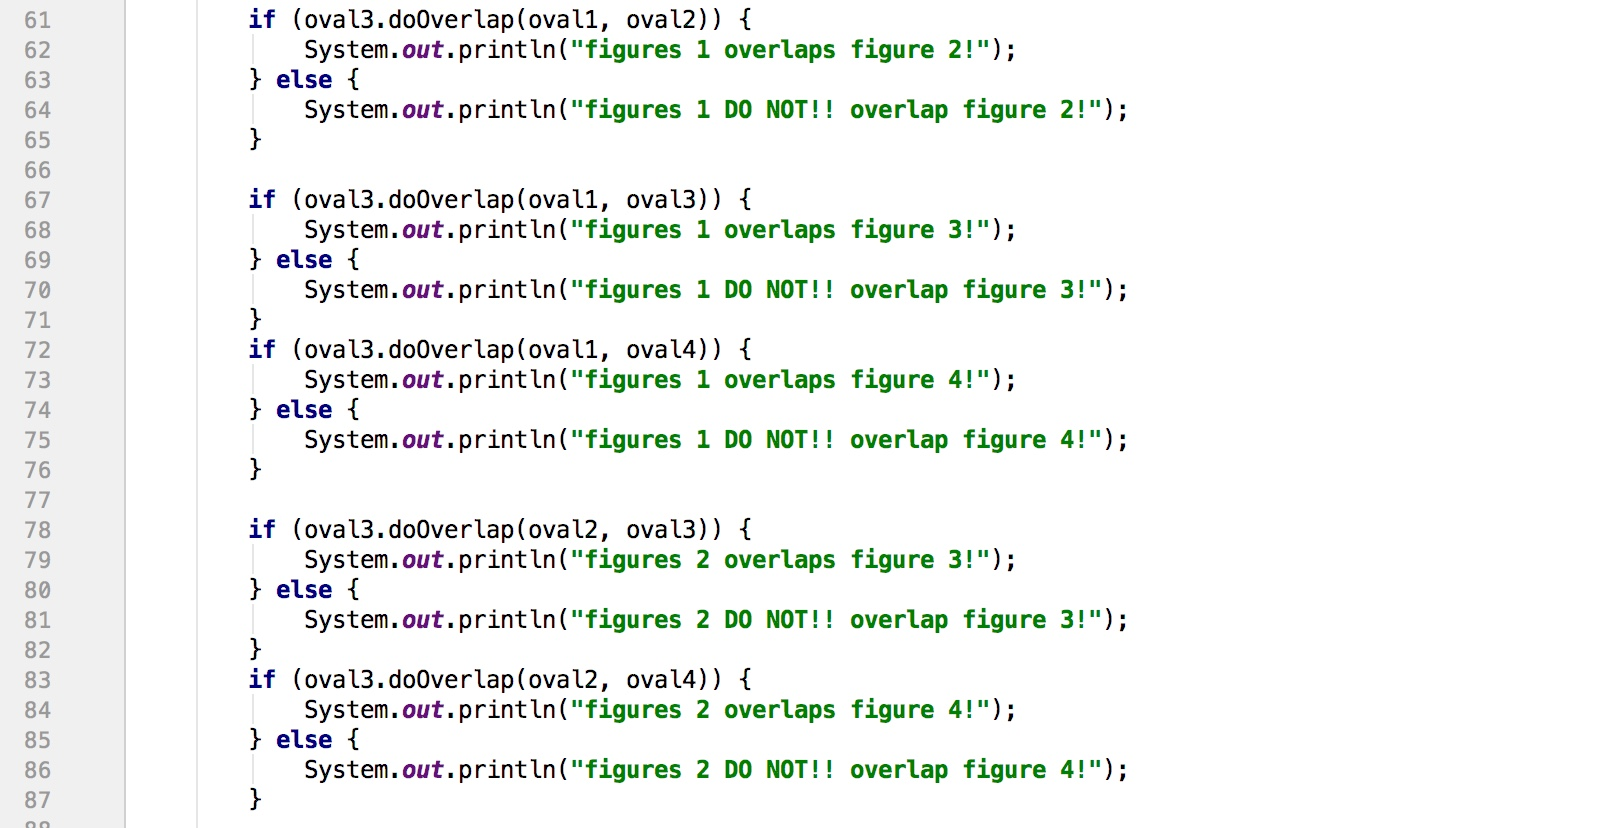
\includegraphics[width = 17cm]{DrawShapesController_for_doOverlap3} % requires the graphicx package
   \caption{DrawShapesController for doOverlap3}
   \label{DrawShapesController for doOverlap3}
\end{figure}

\section{Outputs}



The outputs of code from figures \ref{DrawShapesController for Polymorphism1},\ref{DrawShapesController for Polymorphism2}, \ref{DrawShapesController for Polymorphism3} are shown in figures from \ref{Output_of_DrawShapesController for Polymorphism} to \ref{Output of DrawShapesController for Polymorphism_written2}.


\begin{figure}[H]
   \centering
   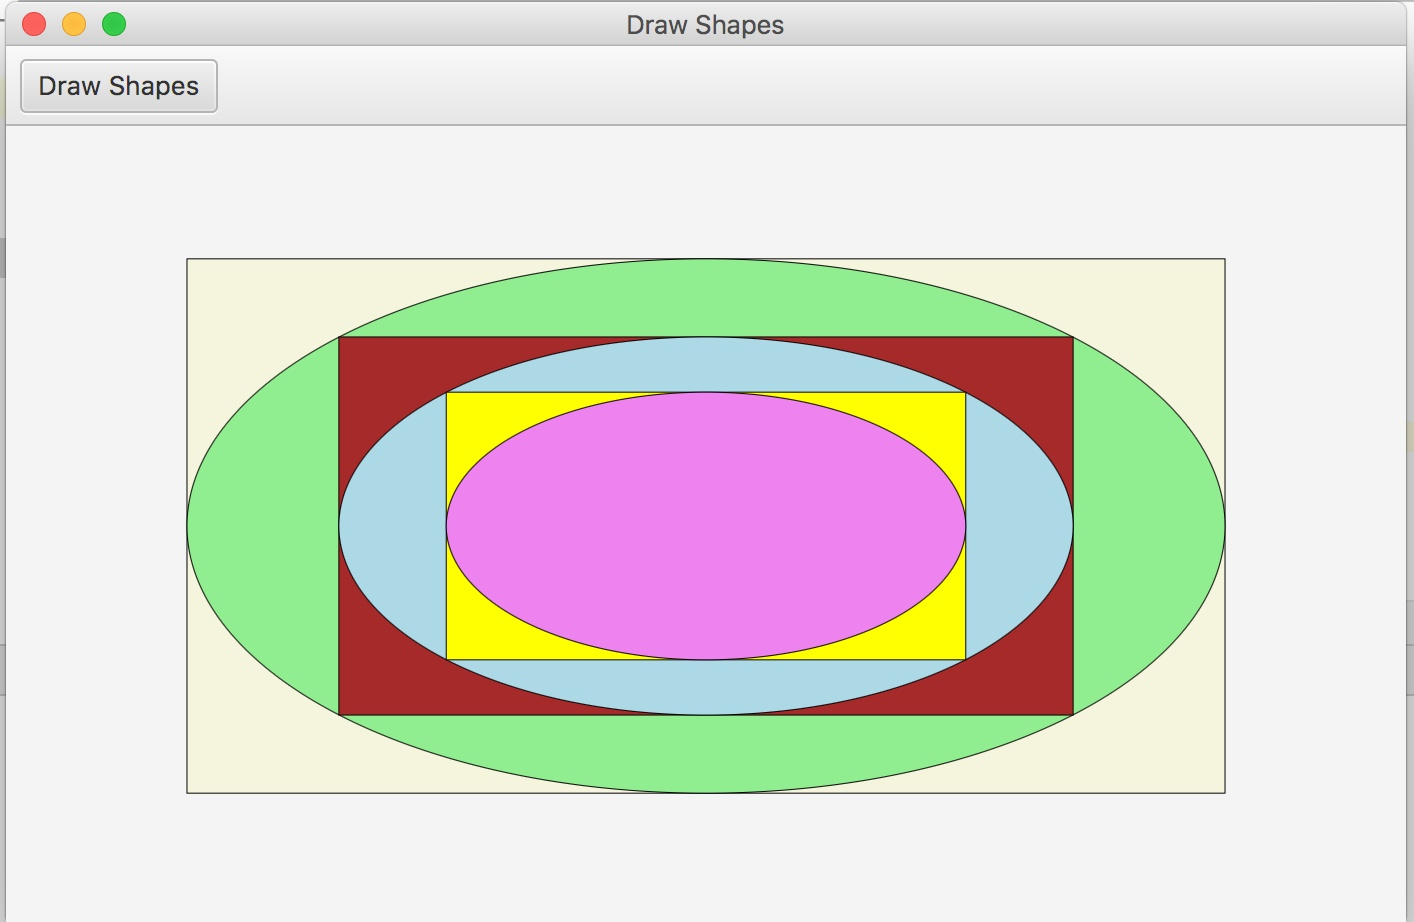
\includegraphics[width = 17cm]{geometric_configuration1} % requires the graphicx package
   \caption{Output of DrawShapesController for Polymorphism}
   \label{Output_of_DrawShapesController for Polymorphism}
\end{figure}


\begin{figure}[H]
   \centering
   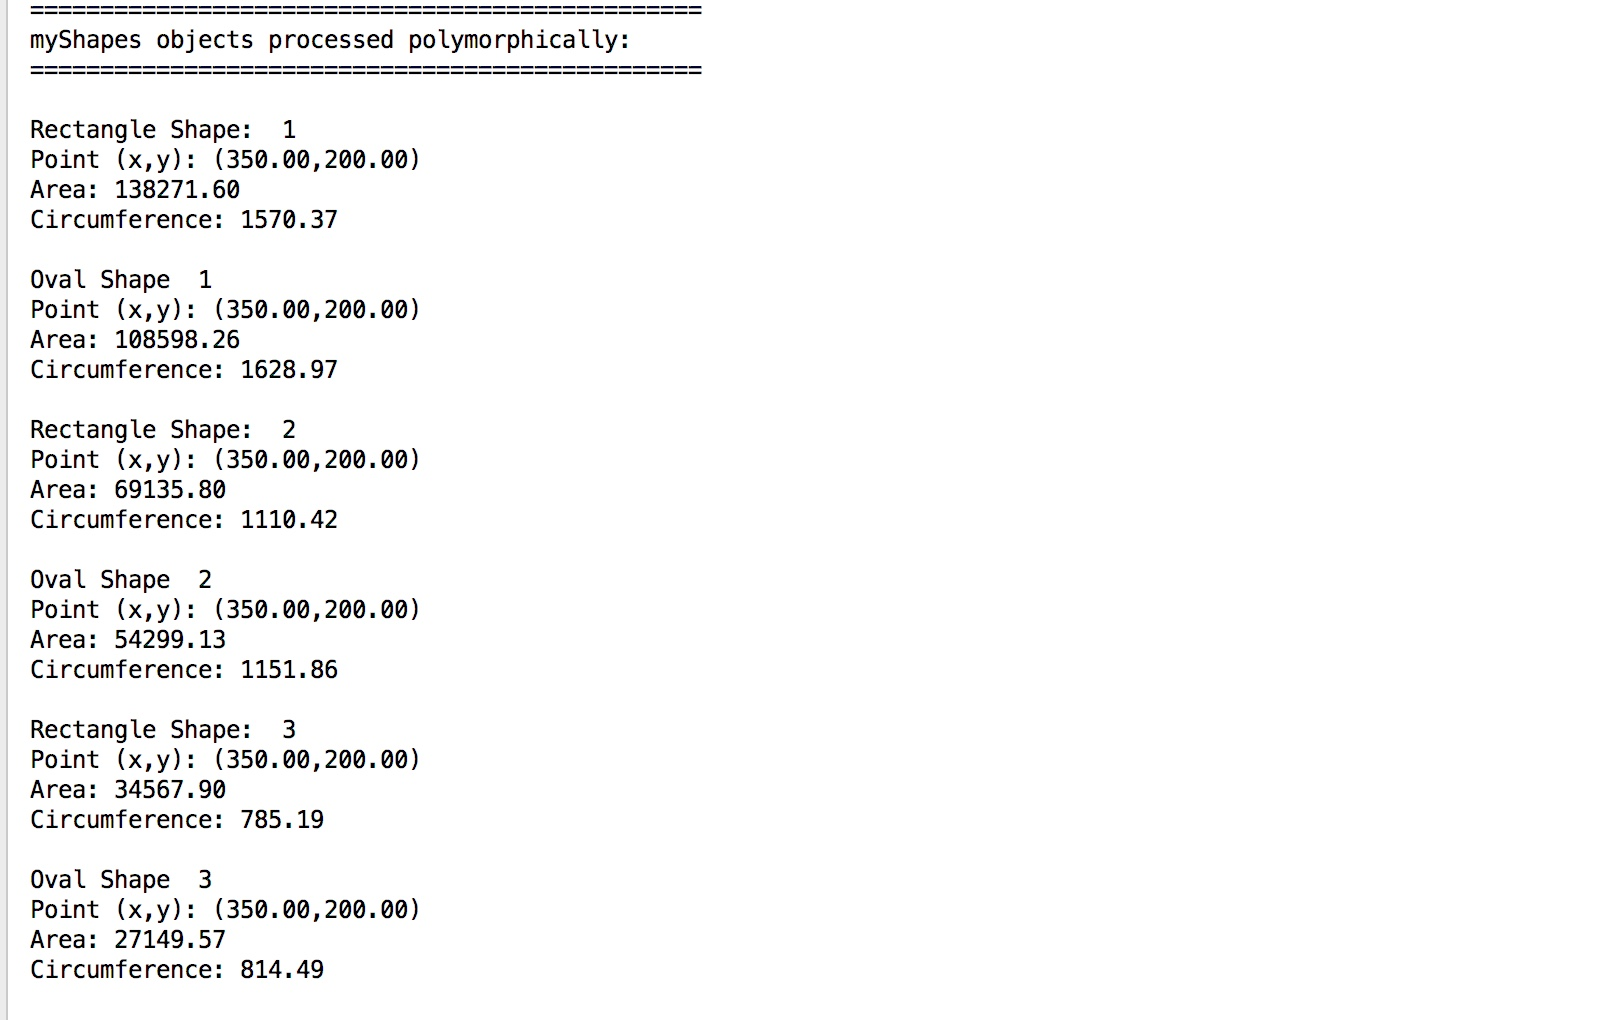
\includegraphics[width = 17cm]{geometric_configuration_written1} % requires the graphicx package
   \caption{Output of DrawShapesController for Polymorphism}
   \label{Output of DrawShapesController for Polymorphism_written}
\end{figure}


\begin{figure}[H]
   \centering
   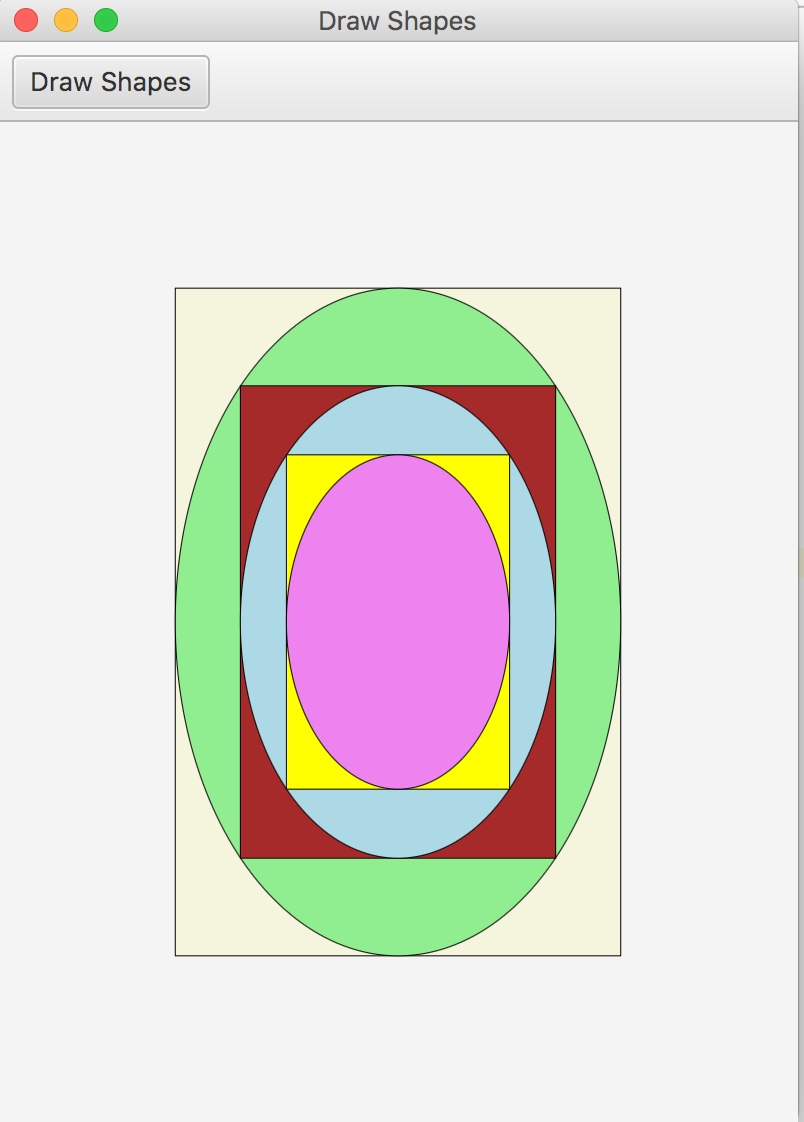
\includegraphics[width = 17cm]{geometric_configuration2} % requires the graphicx package
   \caption{Output of DrawShapesController for Polymorphism}
   \label{Output_of_DrawShapesController for Polymorphism2}
\end{figure}


\begin{figure}[H]
   \centering
   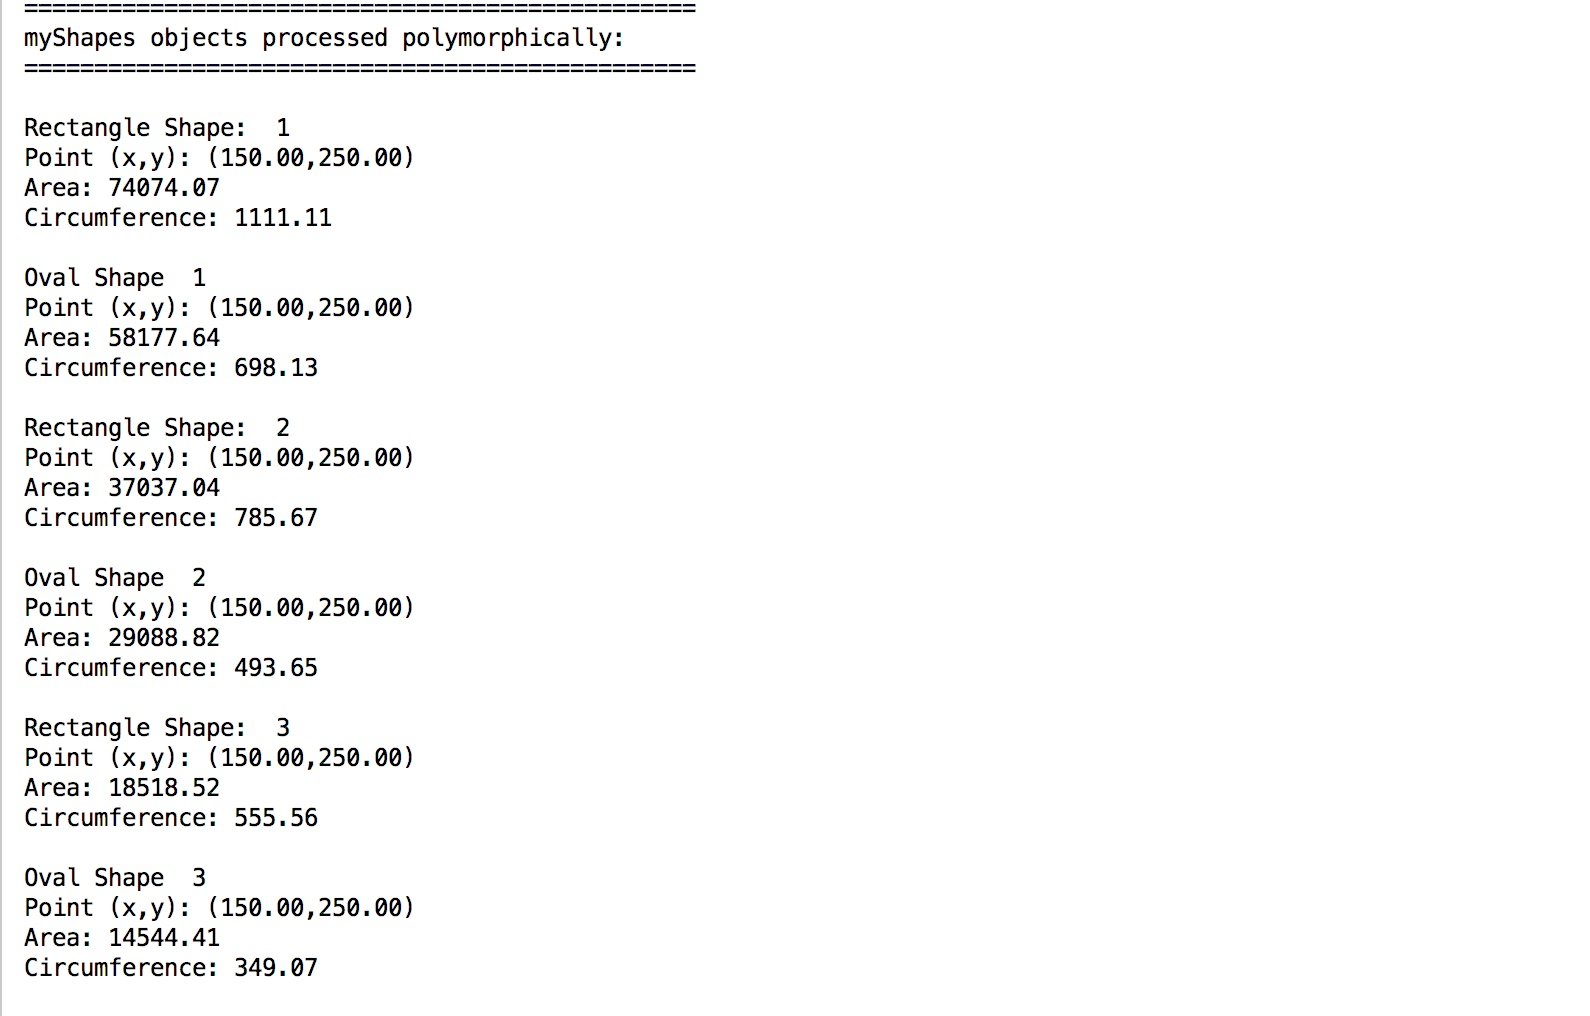
\includegraphics[width = 17cm]{geometric_configuration_written2} % requires the graphicx package
   \caption{Output of DrawShapesController for Polymorphism}
   \label{Output of DrawShapesController for Polymorphism_written2}
\end{figure}



\subsection{doOverlap Test results}
The results of codes  \ref{DrawShapesController for doOverlap1}, \ref{DrawShapesController for doOverlap2}, \ref{DrawShapesController for doOverlap3} are shown in figures \ref{geometric configuration doOverlap}, and 
\ref{geometric configuration doOverlap written }.

\begin{figure}[H]
   \centering
   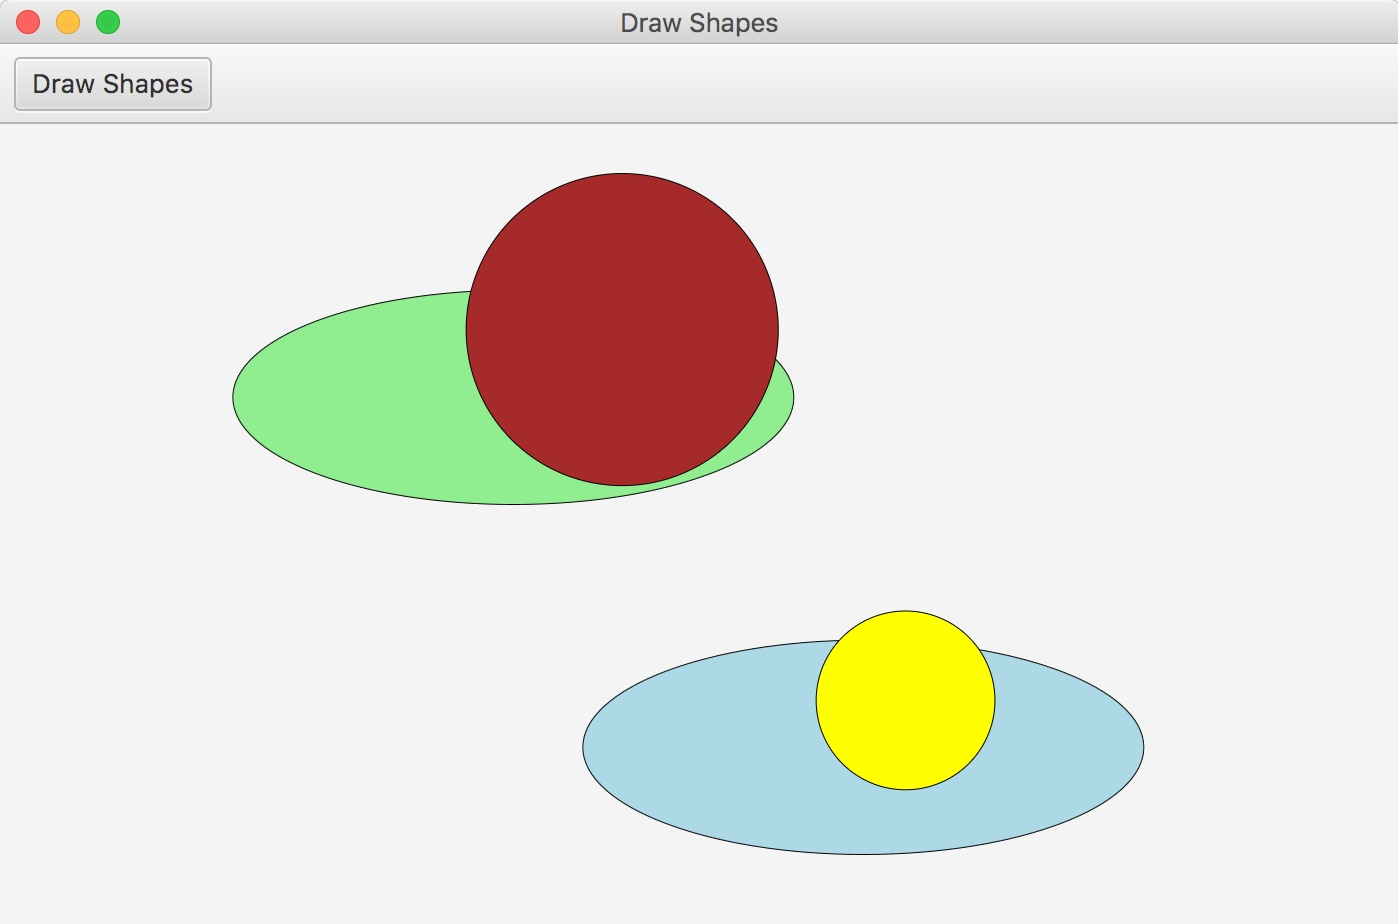
\includegraphics[width = 17cm]{geometric_configuration_do_overlap} % requires the graphicx package
   \caption{geometric configuration doOverlap}
   \label{geometric configuration doOverlap}
\end{figure}


\begin{figure}[H]
   \centering
   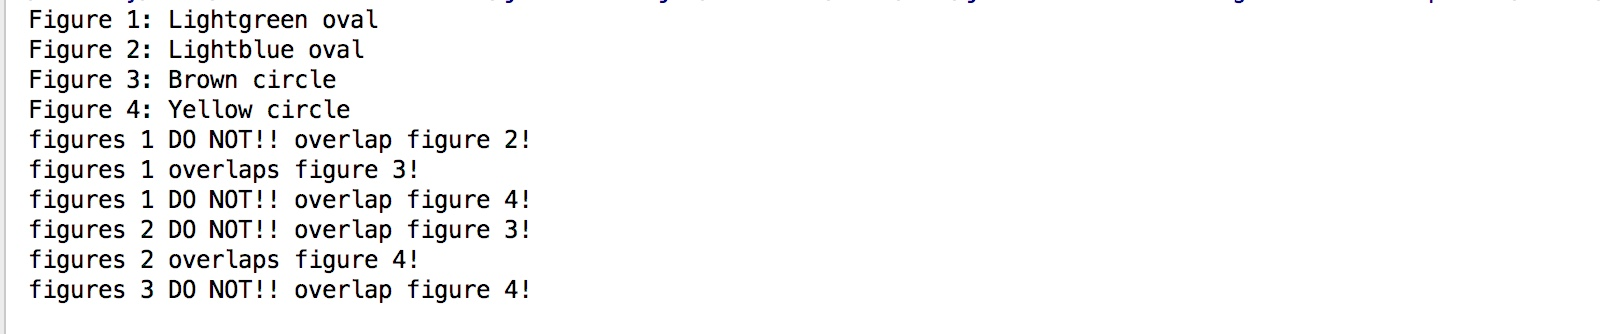
\includegraphics[width = 17cm]{geometric_configuration_do_overlap_written} % requires the graphicx package
   \caption{geometric configuration doOverlap written}
   \label{geometric configuration doOverlap written }
\end{figure}













% ==========% ==========% ==========% ==========% ==========
\newpage
\section{References}
[1]  Deitel, Paul J., and Harvey M. Deitel. Java: How to Program Early Objects. Pearson, 2018.
\end{document}